\lstinputlisting[language=bash,basicstyle=\small]{python_codes/fieldstone_55/keywords}

\begin{center}
\url{https://github.com/cedrict/fieldstone/tree/master/python_codes/fieldstone_55}
\end{center}

\par\noindent\rule{\textwidth}{0.4pt}

{\sl This stone was developed in collaboration with Erik van der Wiel and Neil Ribe}. 
\index{contributors}{E. van der Wiel}
\index{contributors}{N. Ribe}

\par\noindent\rule{\textwidth}{0.4pt}

%--------------------------------------------------------


\vspace{1cm}

Parameters for the setup are defined in {\sl parameters.py}.
This file is used in {\sl generate\_nodes.py} which produces the
{\sl subd.node} file which contains the coordinates of all key points 
on the boundary of the domain and along the material interfaces.
This file is then further processed by the triangle 
program\footnote{\url{https://www.cs.cmu.edu/~quake/triangle.html}}
as follows:
\begin{verbatim}
./triangle -q -a200000000 -o2 subd.node
\end{verbatim}
The '-q' option adds vertices to the mesh to
ensure that all angles are between 20 and 140 degrees. 
The '-a' makes sure that no triangle has an area larger than 
the supplied number. The '-o2' generates a mesh composed 
of second order triangles (six nodes per element, rather than three) and the
three extra nodes of an element fall at the midpoints of the three edges.
This generates two files: 'subd.1.ele' which contains the connectivity 
of all generated triangles and 'subd.1.node' which contains the coordinates
of all nodal points. 
These two files are then read in {\sl fieldstone.py} and stored in the xV, yV and iconV arrays.

Gravity is vertical and Earth-like. Free-slip boundary conditions are imposed on the top while 
the other boundaries are free (in/outflow determined freely based on the internal dynamics). 
Crouzeix-Raviart elements are used, see Section~\ref{sec:crouzeix-raviart}.
The density of the mantle is set to zero while the subducting plate has a density $\delta\rho$. 

In order to remove the horizontal null space (when the side boundaries are fully open) 
the average horizontal velocity of the domain is set to zero,
which we will revisit a bit later. Neil wrote: ``The BEM 
solves the nullspace problem naturally because the Green functions
all decay to zero at infinity. That means that the velocity solutions 
are all relative to a state of rest at infinity.''

As an exercise, we can ask ourselves where the center of mass of the slab is located.
If the mass distribution is continuous with the density $\rho(\vec{r})$ 
within a solid $Q$, then the integral of the weighted position coordinates 
of the points in this volume relative to the center of mass $\vec{R}$ over the volume $V$ is zero, 
that is
\[
\iiint_Q \rho(\vec{r}) (\vec{r}-\vec{R}) dV =0
\]
Since the density in the slab is constant this simplifies to 
\[
\iiint_Q  (\vec{r}-\vec{R}) dV =0
\]
or, 
\[
\vec{R} = \frac{ \iiint_Q  \vec{r} dV}{\iiint_Q  dV}
\]
We find $\vec{R}=(940.7808, 873.6642)km$ for a 2000x1000km domain.




\begin{center}
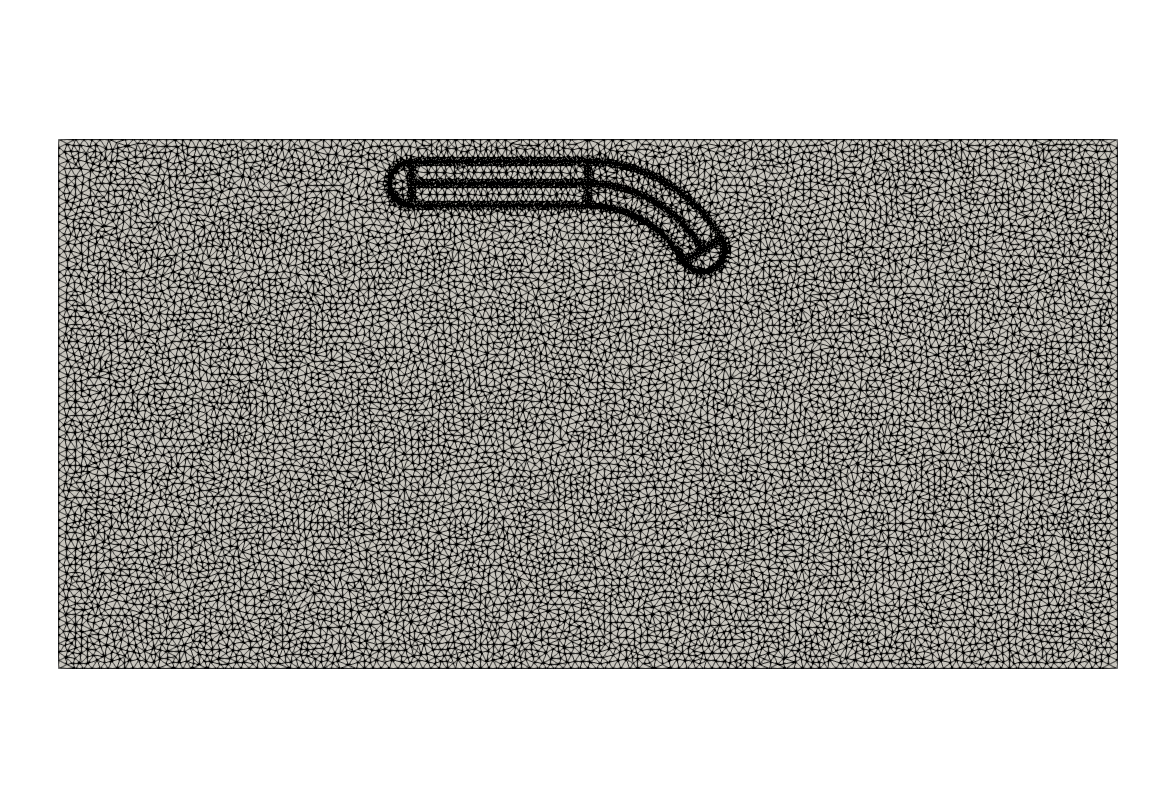
\includegraphics[width=7.75cm]{python_codes/fieldstone_55/images/mesh}
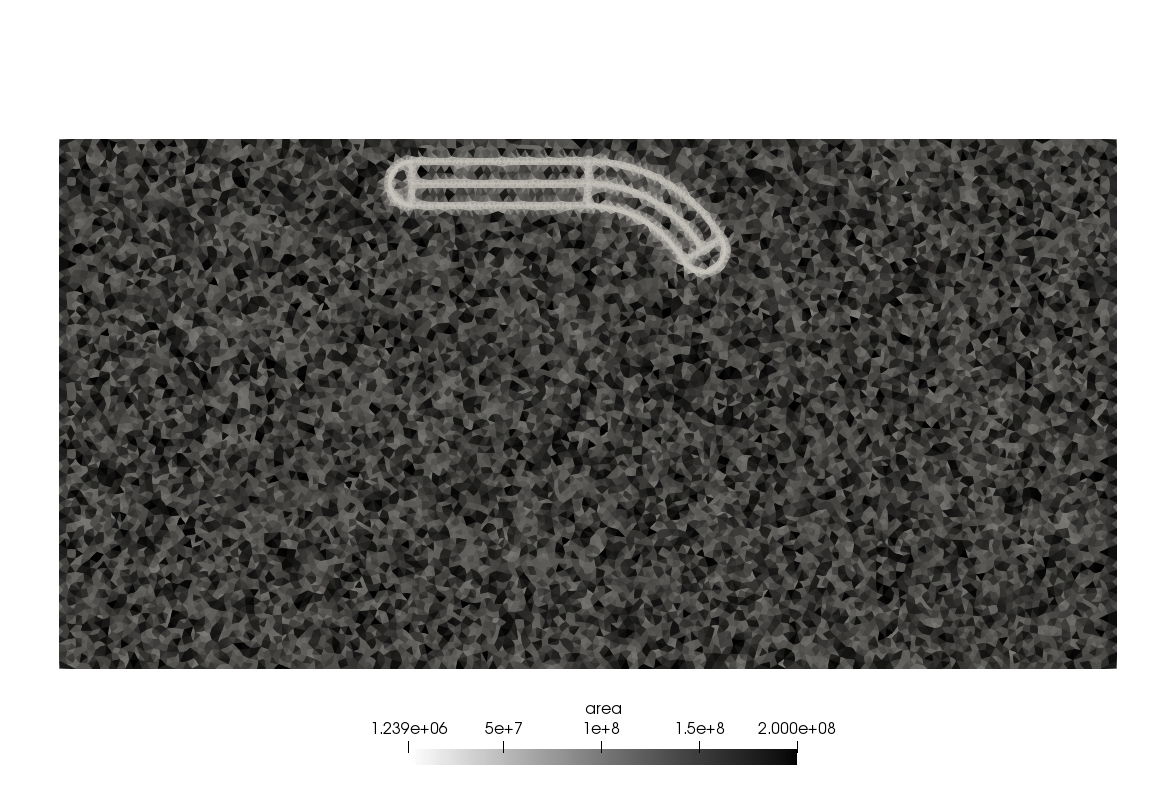
\includegraphics[width=7.75cm]{python_codes/fieldstone_55/images/area}\\
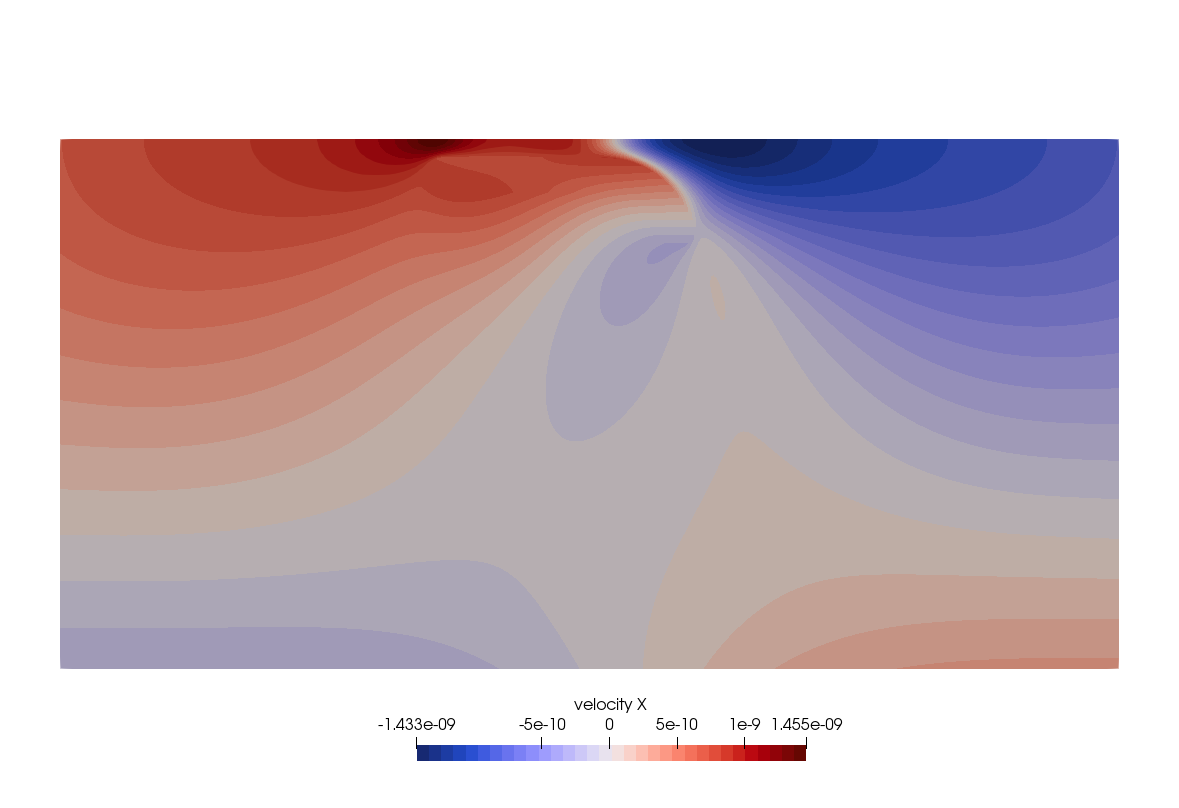
\includegraphics[width=7.75cm]{python_codes/fieldstone_55/images/u}
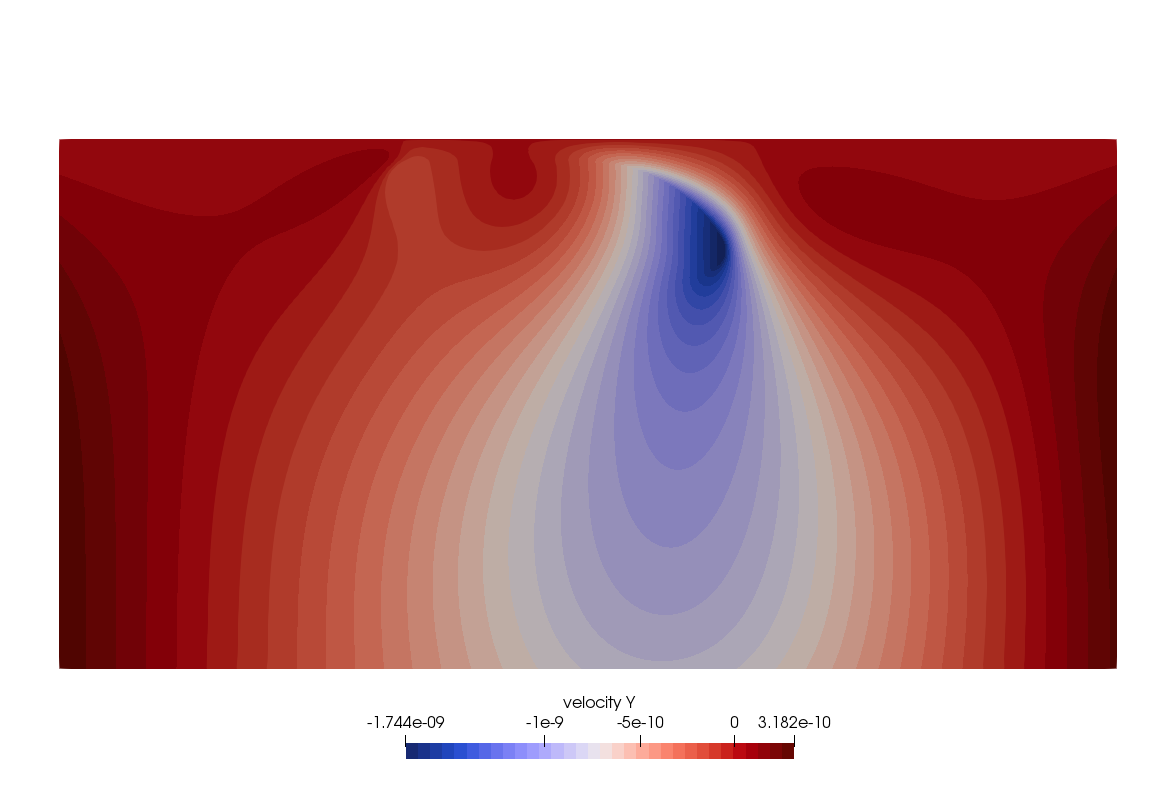
\includegraphics[width=7.75cm]{python_codes/fieldstone_55/images/v}\\
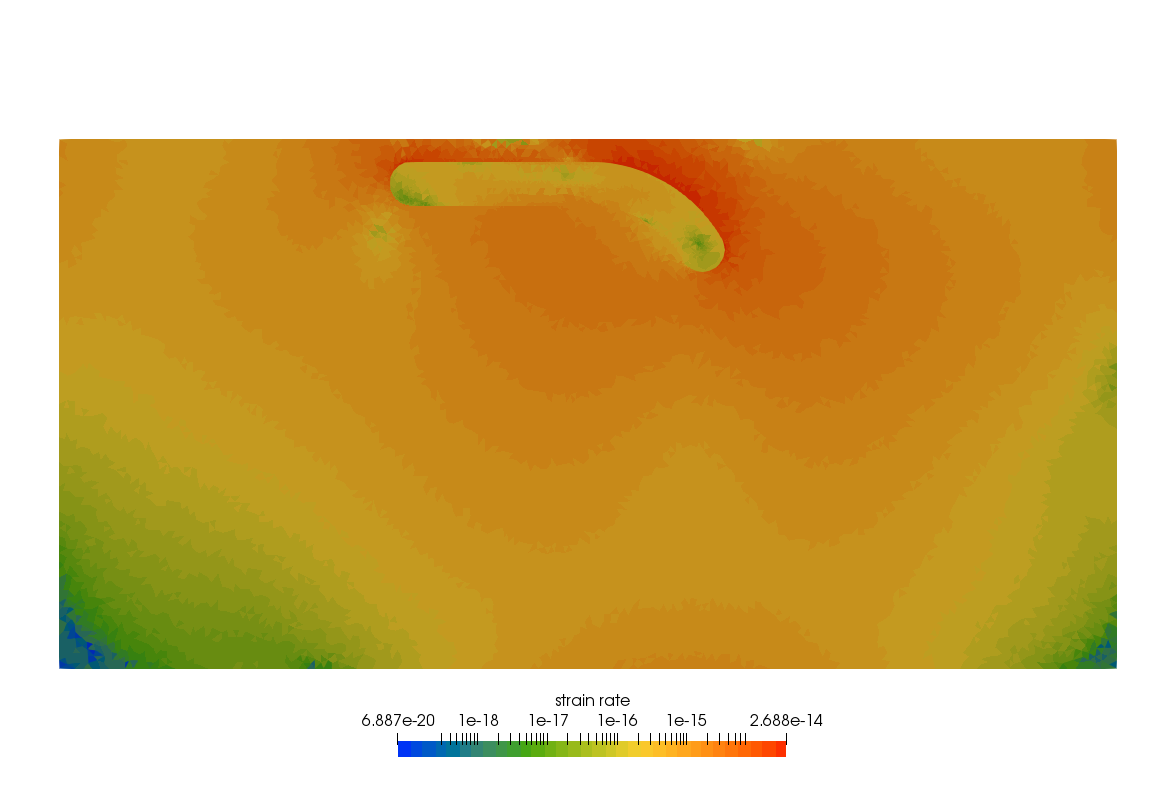
\includegraphics[width=7.75cm]{python_codes/fieldstone_55/images/sr}
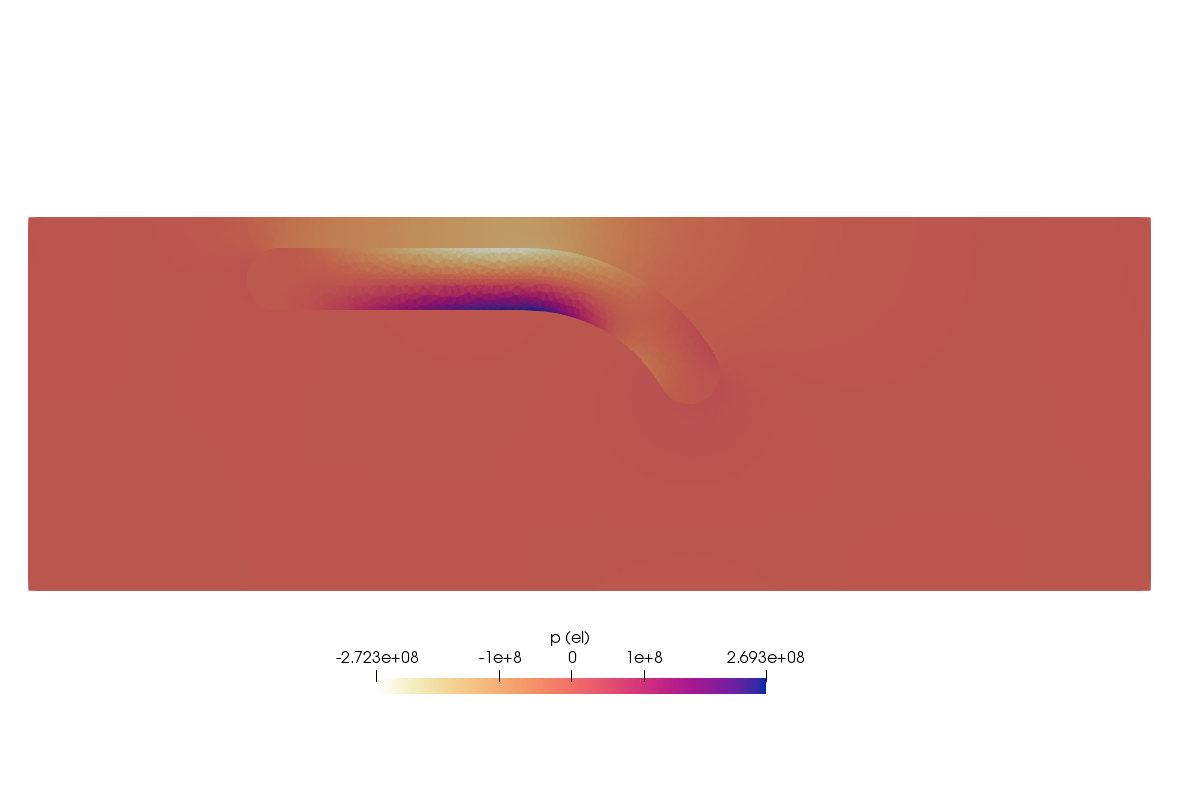
\includegraphics[width=7.75cm]{python_codes/fieldstone_55/images/press}\\
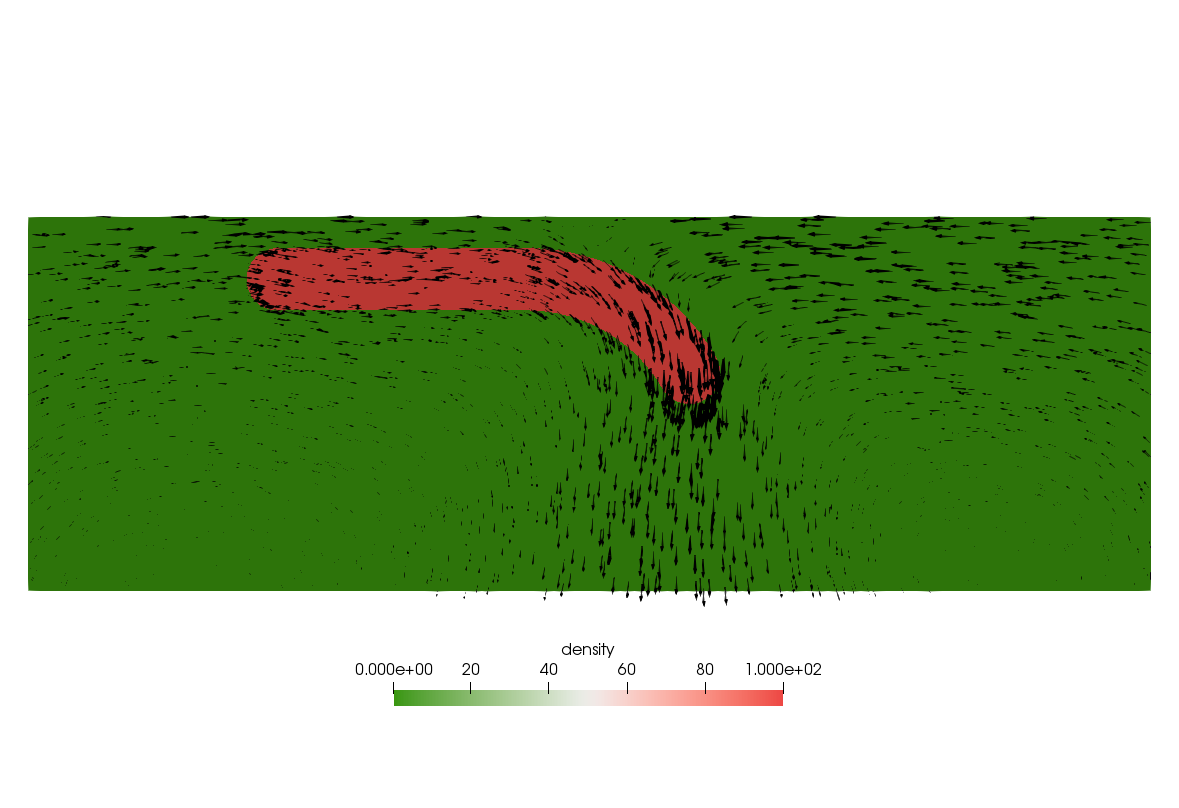
\includegraphics[width=7.75cm]{python_codes/fieldstone_55/images/rho}
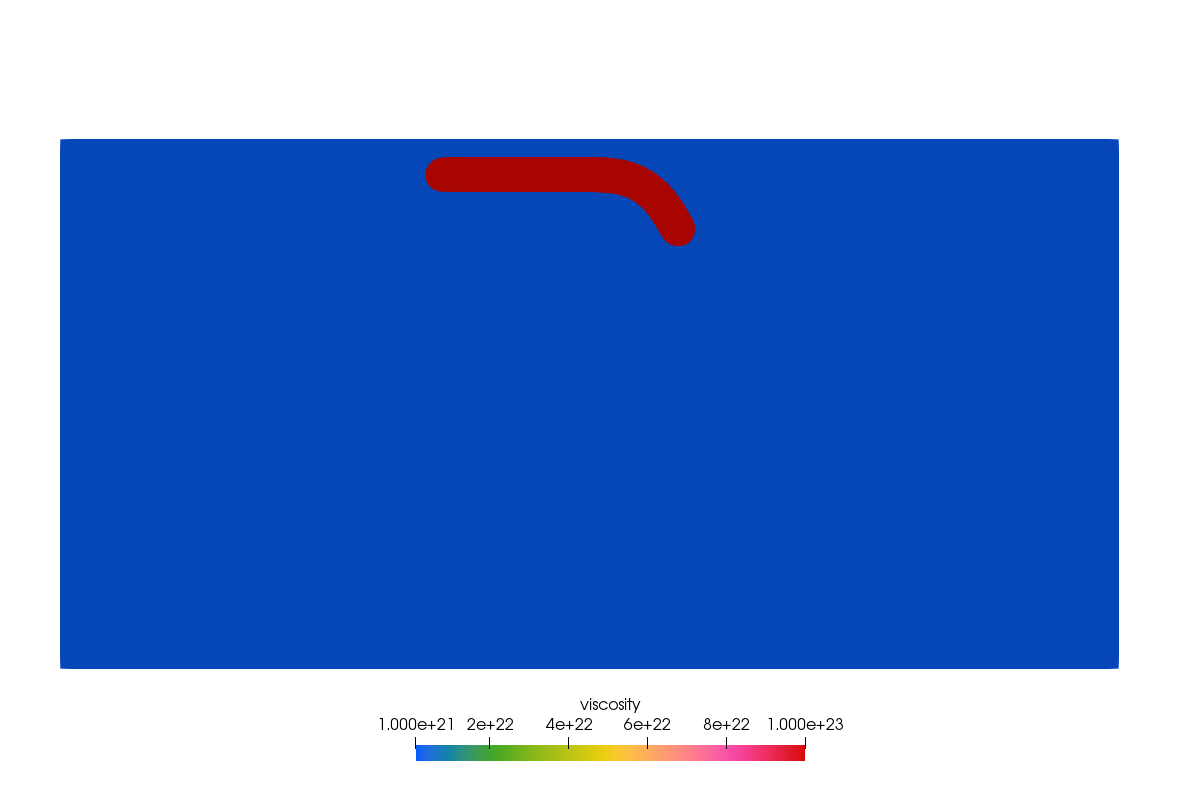
\includegraphics[width=7.75cm]{python_codes/fieldstone_55/images/eta}\\
{\captionfont Mesh composed of 31,765 triangles.
Other parameters: $\theta_0=60\degree$, $\eta_1=10^{21}$, $\gamma=100$, 
$L_x$=3000km, $L_y$=1500km, $\delta\rho=100$, $L=$400km, $h=$100km, $d=$50km. 
Note that the bottom boundary is open.}
\end{center}

%\begin{center}
%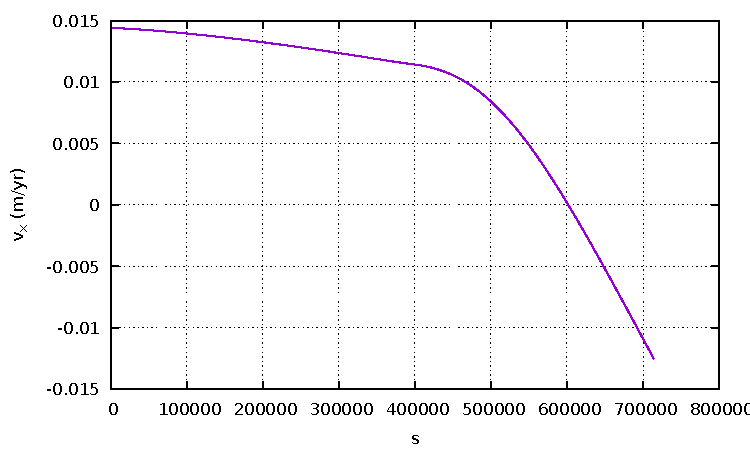
\includegraphics[width=5cm]{python_codes/fieldstone_55/images/spine_u}
%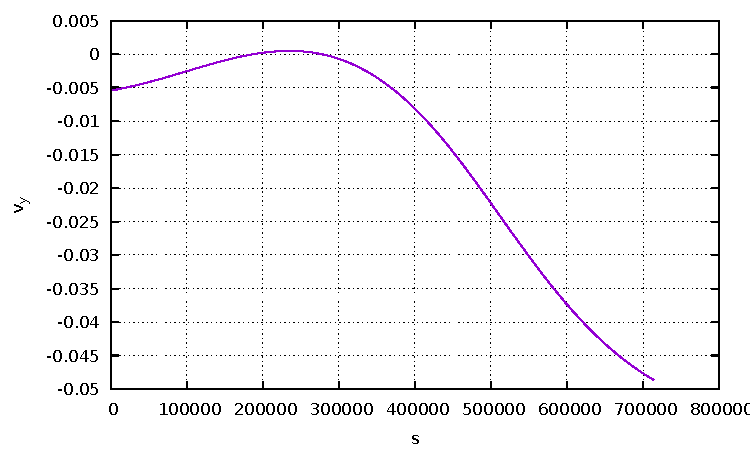
\includegraphics[width=5cm]{python_codes/fieldstone_55/images/spine_v}
%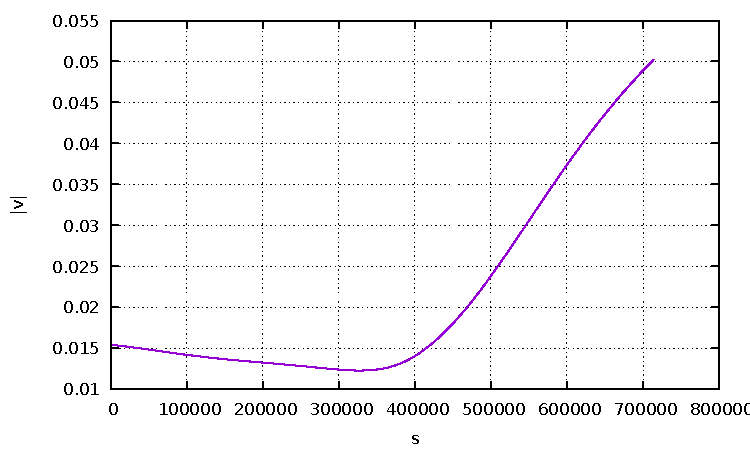
\includegraphics[width=5cm]{python_codes/fieldstone_55/images/spine_vel}\\
%{\scriptsize horizontal and vertical velocity, and velocity norm as a function 
%of $s$. $s$ is measured from 
%left to right on the midsurface and excludes the rounded edges of the slab.}
%\end{center}

We have also run this model with ASPECT for the case where free slip 
boundary conditions are prescribed on all sides. 
Velocities on the midsurface are reported hereunder alongside those
obtained with fieldstone and the BEM method.

\begin{center}
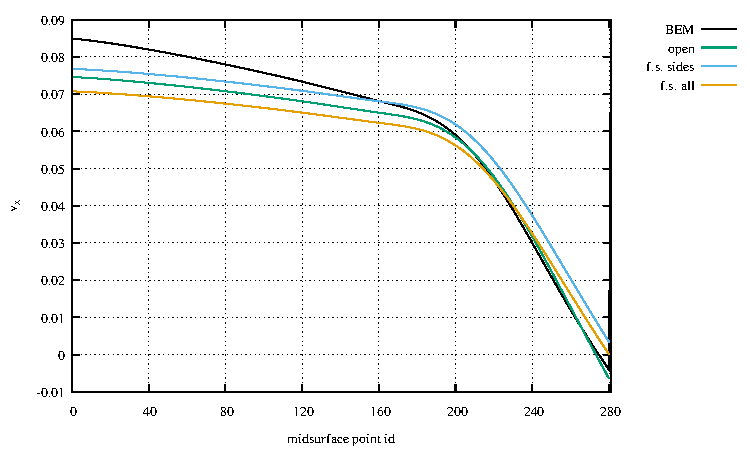
\includegraphics[width=7.5cm]{python_codes/fieldstone_55/images/u_midsurface}
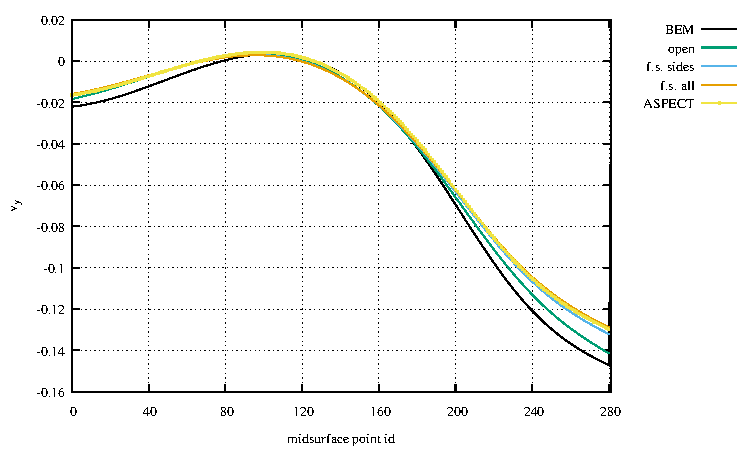
\includegraphics[width=7.5cm]{python_codes/fieldstone_55/images/v_midsurface}\\
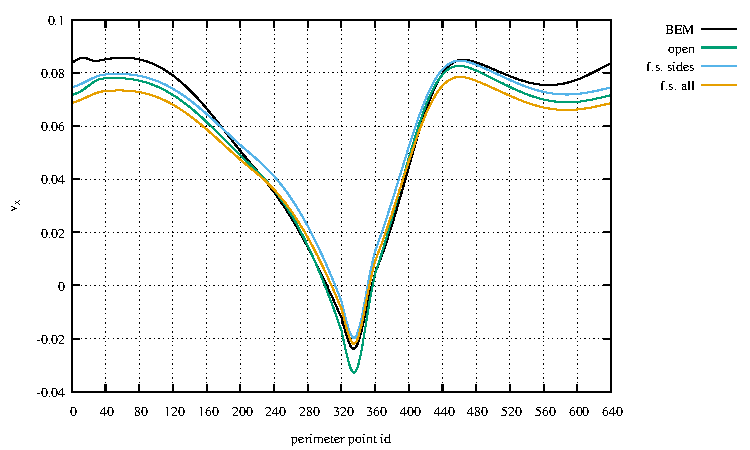
\includegraphics[width=7.5cm]{python_codes/fieldstone_55/images/u_perimeter}
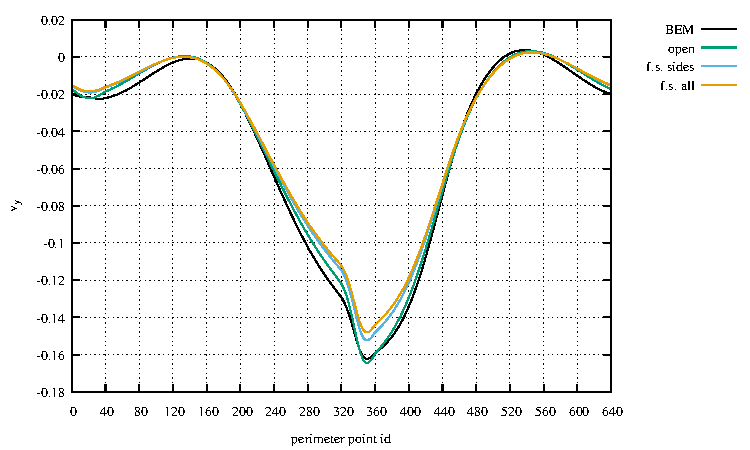
\includegraphics[width=7.5cm]{python_codes/fieldstone_55/images/v_perimeter}\\
{\captionfont Top row: midsurface velocity measurements. Bottom row: slab/plate perimeter 
velocity measurements. 'open' means no b.c. on sides and bottom; 'f.s. sides' means 
free slip b.c. on left and right sides, open at the bottom; 'f.s. all' means 
free slip b.c. on sides and bottom.}
\end{center}

\newpage
%----------------------------------------------------------------------
\subsection*{Exploring the influence of the domain size}

The BEM method is such that the domain is actually a semi-infinite plane.
All I can do in a FEM code is prescribe no kinematic boundary conditions on the side and bottom 
boundaries and use a 'large enough' domain. But what is large enough? Let us investigate.

I have explored domains from size 2000x1000 up to 6000x3000 km. 
The slab remains at the same location below the surface and in the middle of the domain
in the $x$-direction as shown here:
\begin{center}

\includegraphics[width=5.7cm]{python_codes/fieldstone_55/gamma001/small}
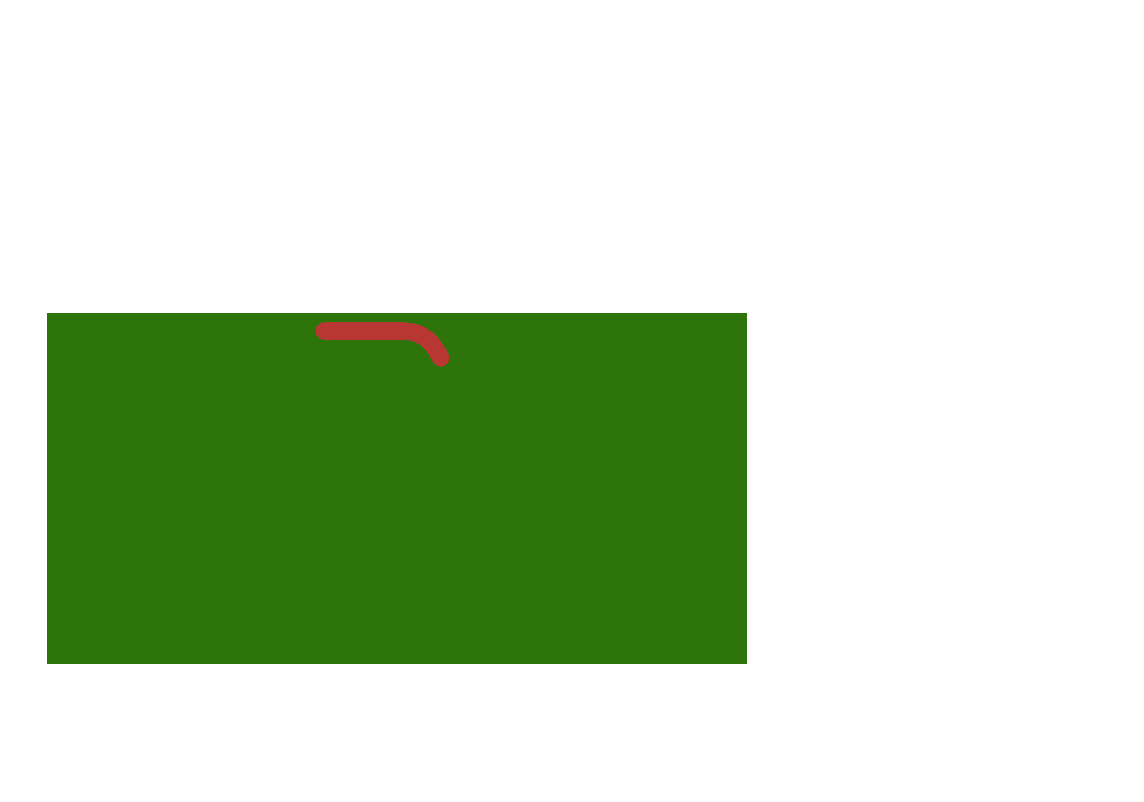
\includegraphics[width=5.7cm]{python_codes/fieldstone_55/gamma001/mid}

\includegraphics[width=5.7cm]{python_codes/fieldstone_55/gamma001/large}\\
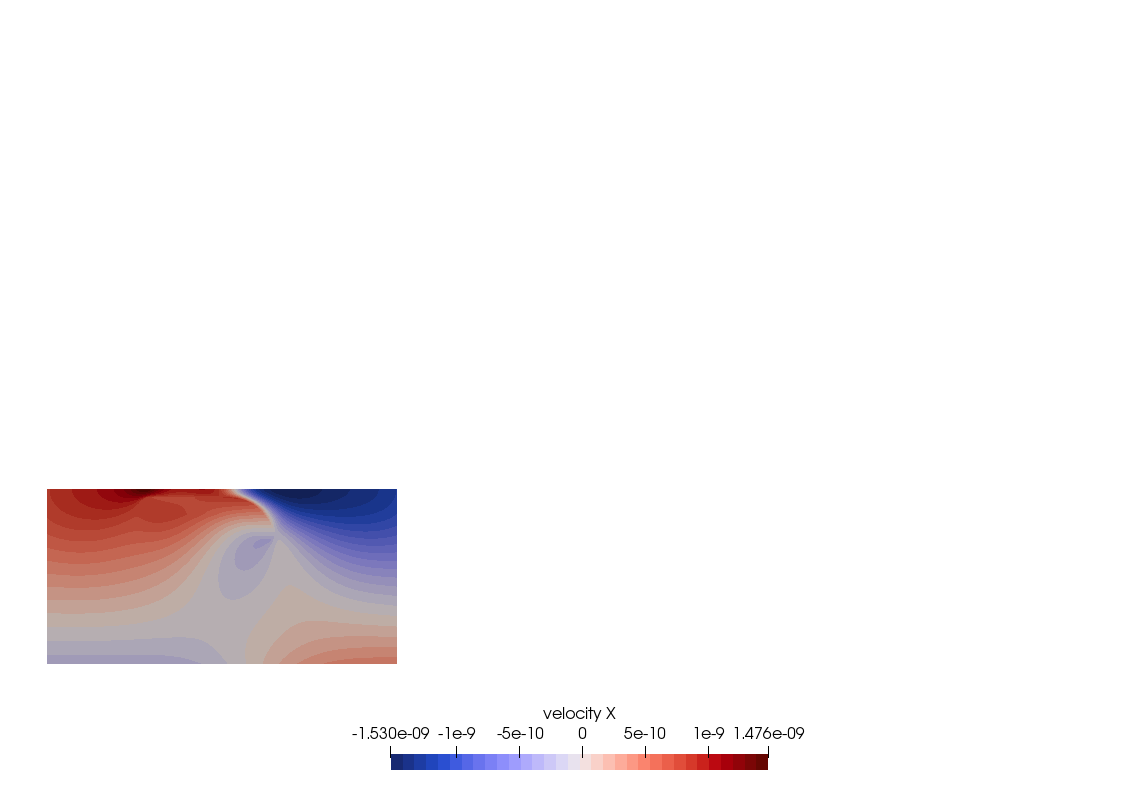
\includegraphics[width=5.7cm]{python_codes/fieldstone_55/gamma100/vx_small}
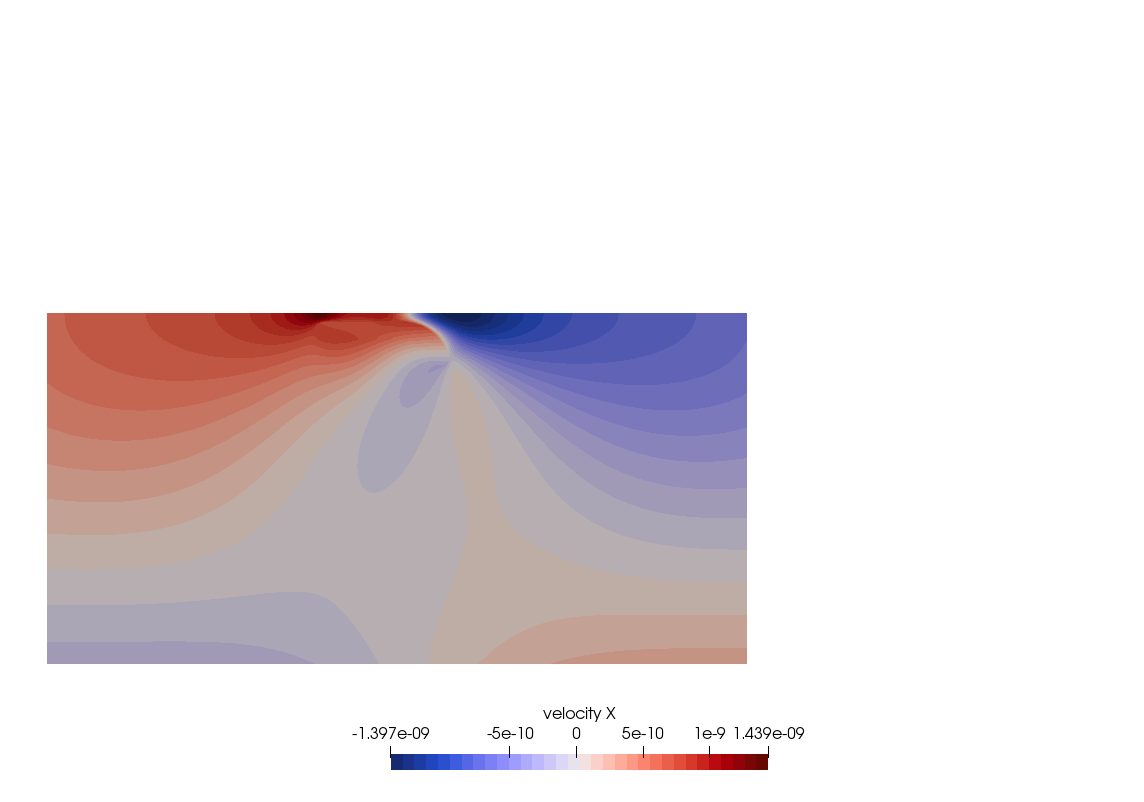
\includegraphics[width=5.7cm]{python_codes/fieldstone_55/gamma100/vx_medium}
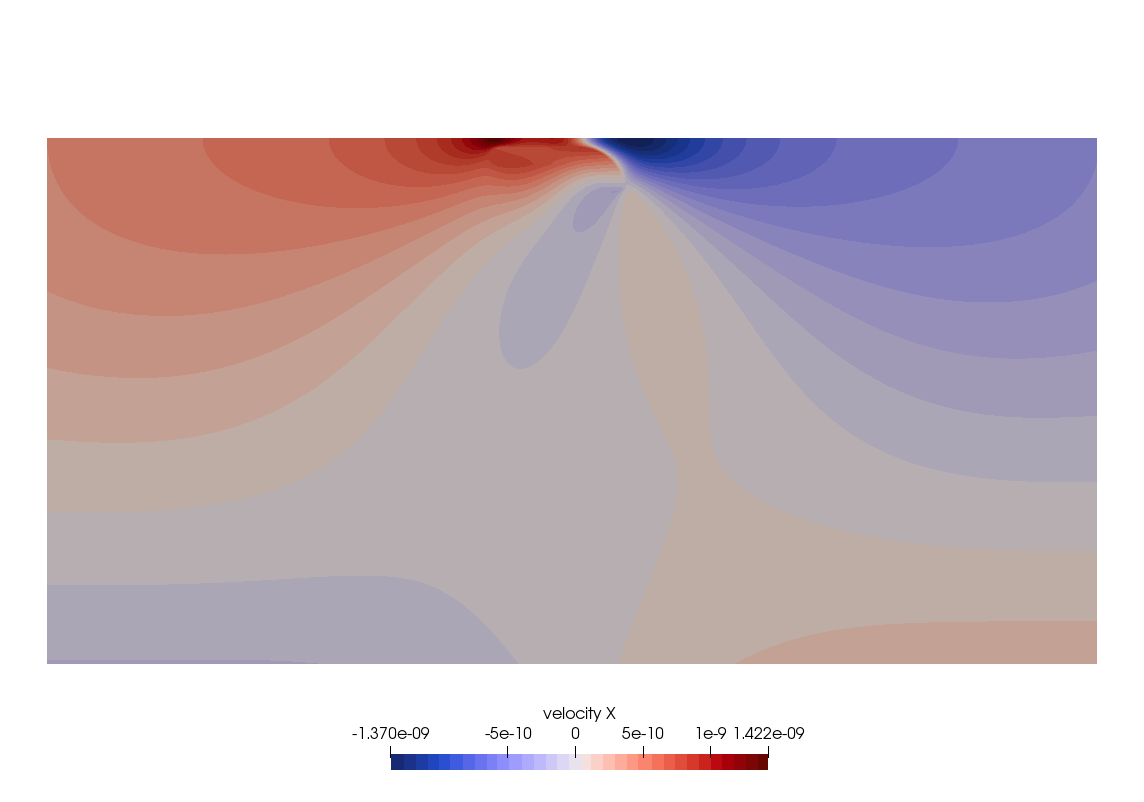
\includegraphics[width=5.7cm]{python_codes/fieldstone_55/gamma100/vx_large}\\
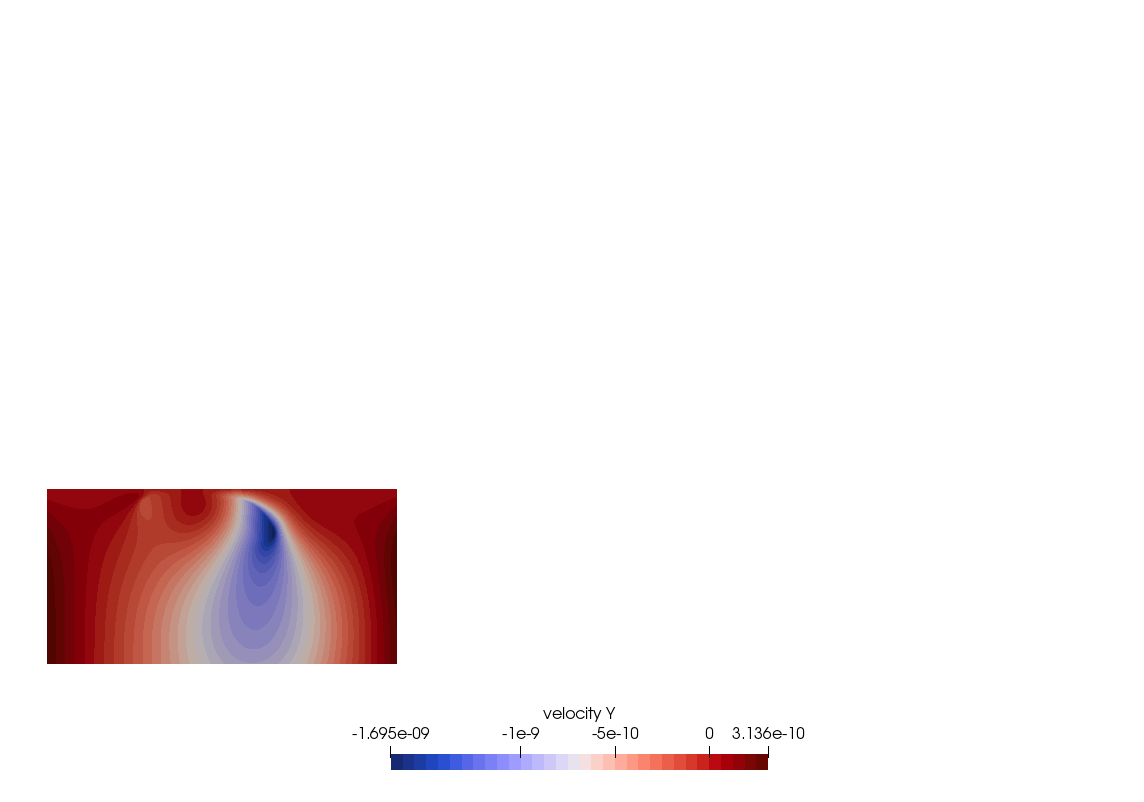
\includegraphics[width=5.7cm]{python_codes/fieldstone_55/gamma100/vy_small}
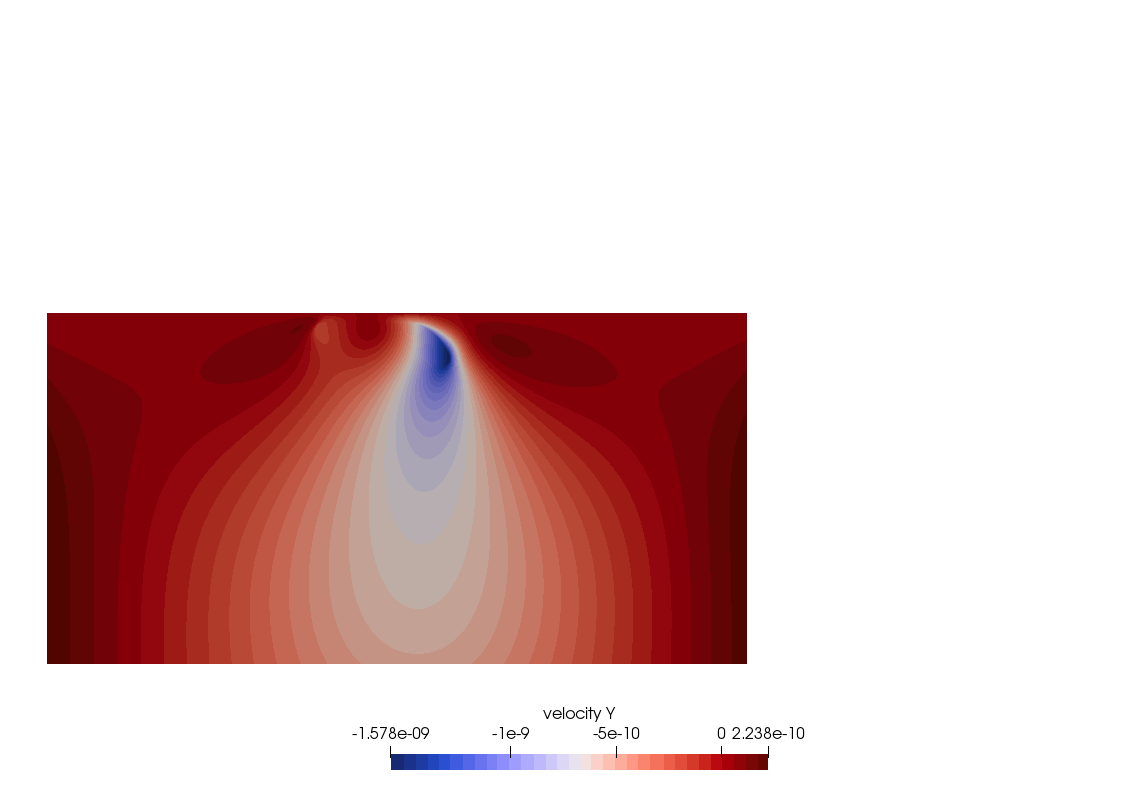
\includegraphics[width=5.7cm]{python_codes/fieldstone_55/gamma100/vy_medium}
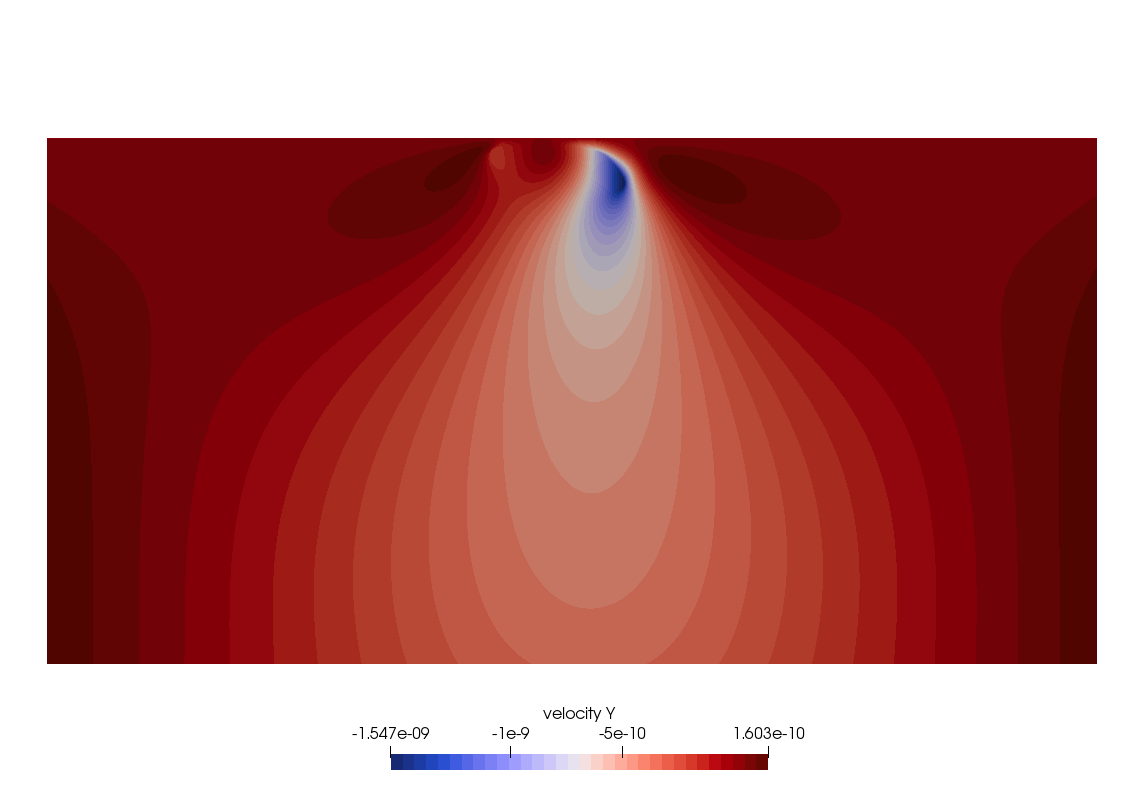
\includegraphics[width=5.7cm]{python_codes/fieldstone_55/gamma100/vy_large}\\
{\captionfont From left to right: 2000x1000, 4000x2000, 6000x3000km domains. Density field.}
\end{center}

I also revisit the null space removal algorithm. Because the domain size changes 
using the total average horizontal velocity makes little sense. Instead 
I compute the average horizontal velocity of the slab only. 

We define also the reference velocity as:
\[
V_{ref}= \frac{h^2 g \delta \rho }{\eta} = \frac{100e3^2 \cdot 9.81 \cdot 100}{1e21}
\]

\begin{center}
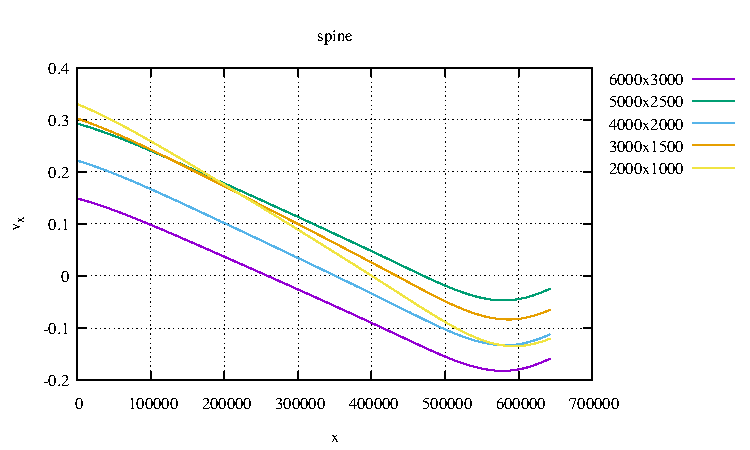
\includegraphics[width=5.7cm]{python_codes/fieldstone_55/gamma001/vx_spine}
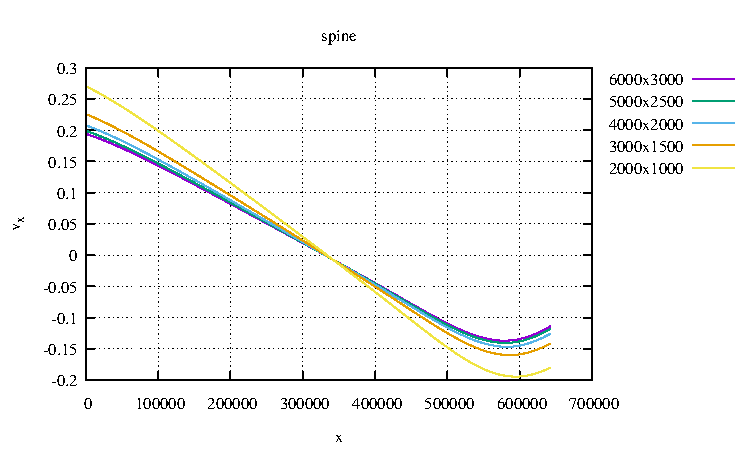
\includegraphics[width=5.7cm]{python_codes/fieldstone_55/gamma001/vx_spine2}
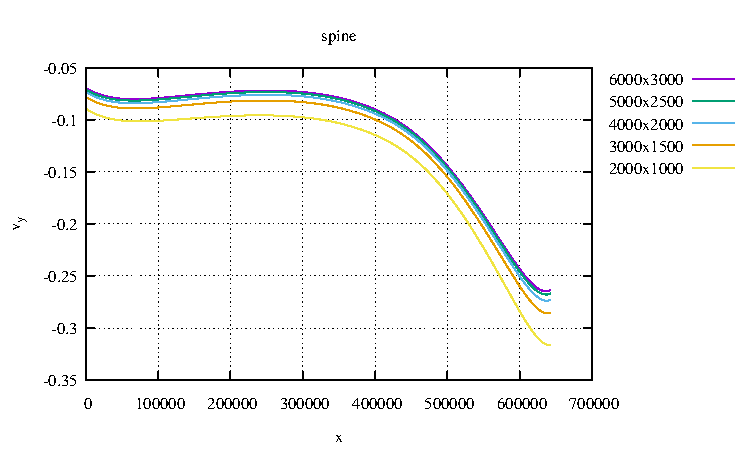
\includegraphics[width=5.7cm]{python_codes/fieldstone_55/gamma001/vy_spine}\\
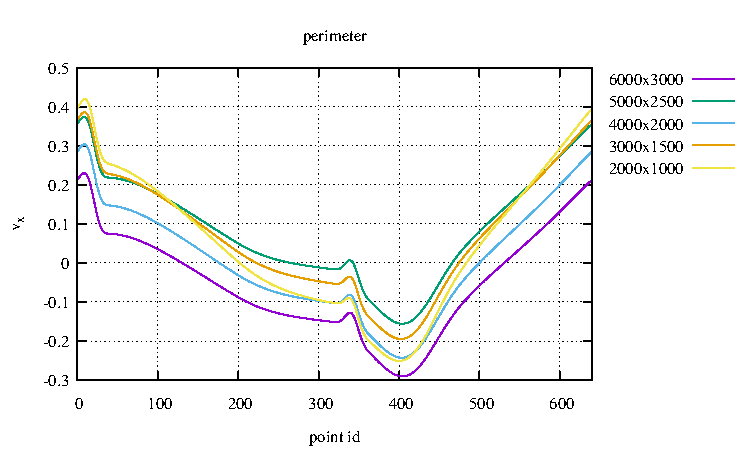
\includegraphics[width=5.7cm]{python_codes/fieldstone_55/gamma001/vx_perimeter}
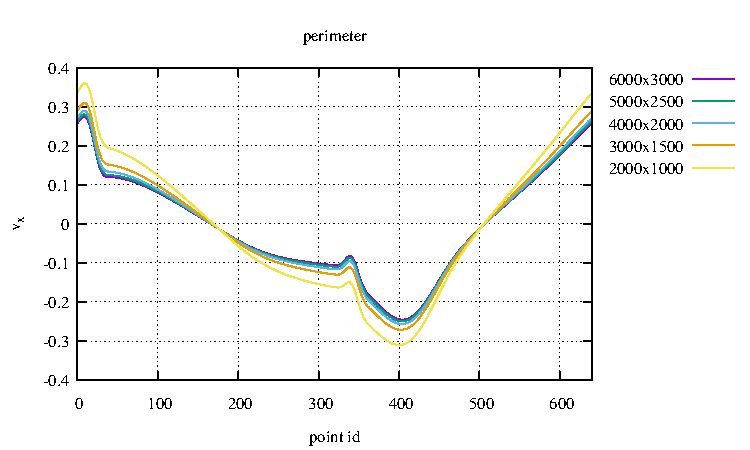
\includegraphics[width=5.7cm]{python_codes/fieldstone_55/gamma001/vx_perimeter2}
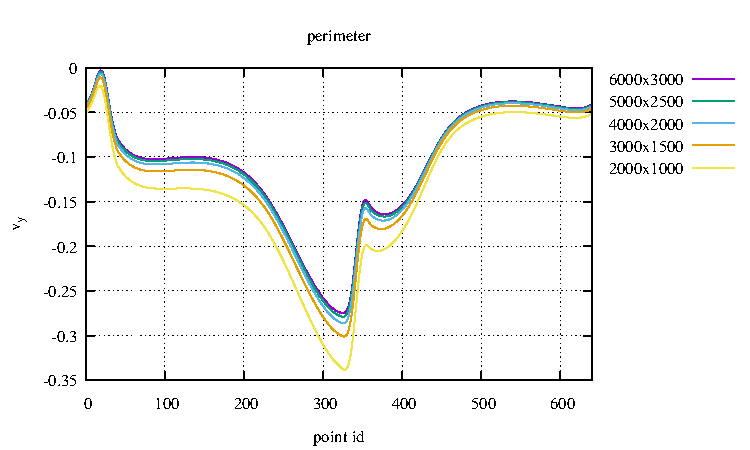
\includegraphics[width=5.7cm]{python_codes/fieldstone_55/gamma001/vy_perimeter}\\
{\captionfont Viscosity contrast $\gamma=1$. From left to right: $u$, zero slab velocity-normalised $u$ 
and $v$ as measured on the spine (top row) and on the perimeter (bottom row). Velocities are normalised by $V_{ref}$}
\end{center}


\begin{center}
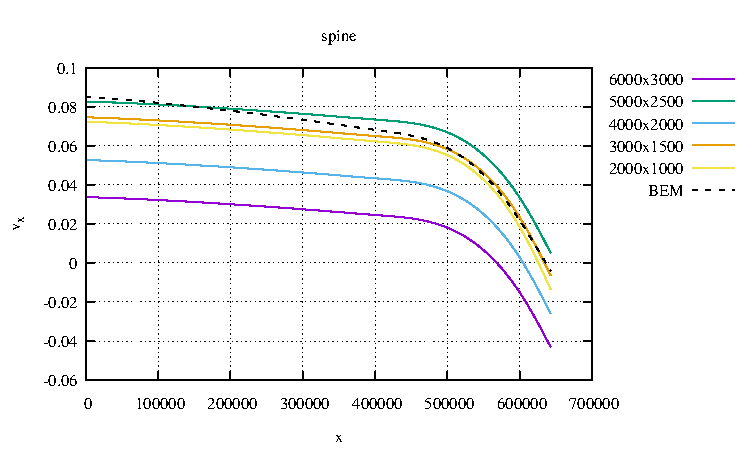
\includegraphics[width=5.7cm]{python_codes/fieldstone_55/gamma100/vx_spine}
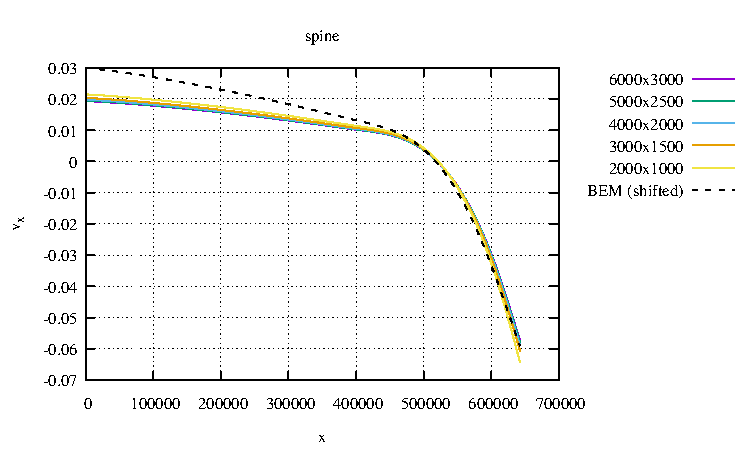
\includegraphics[width=5.7cm]{python_codes/fieldstone_55/gamma100/vx_spine2}
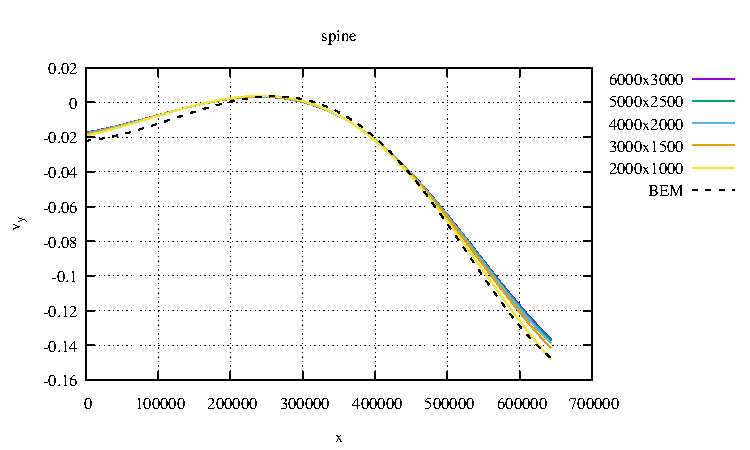
\includegraphics[width=5.7cm]{python_codes/fieldstone_55/gamma100/vy_spine}\\
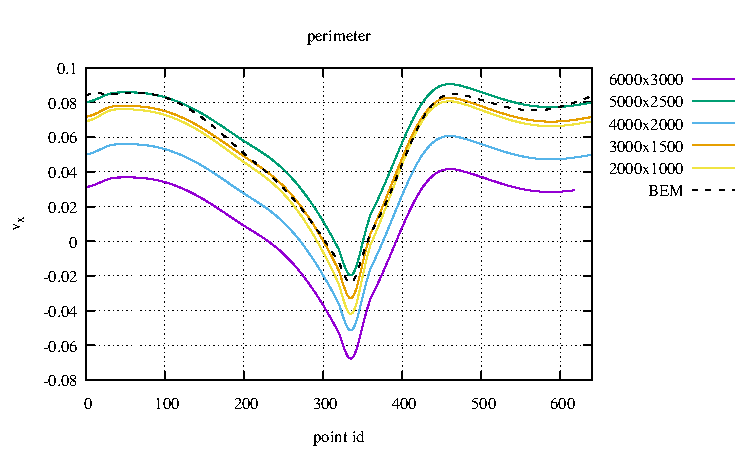
\includegraphics[width=5.7cm]{python_codes/fieldstone_55/gamma100/vx_perimeter}
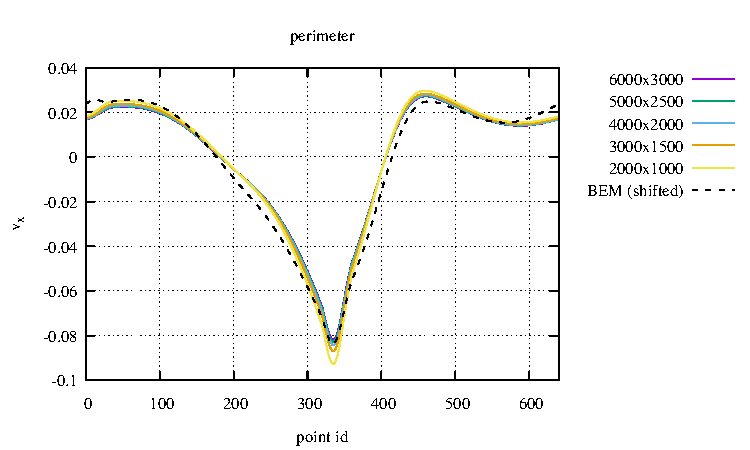
\includegraphics[width=5.7cm]{python_codes/fieldstone_55/gamma100/vx_perimeter2}
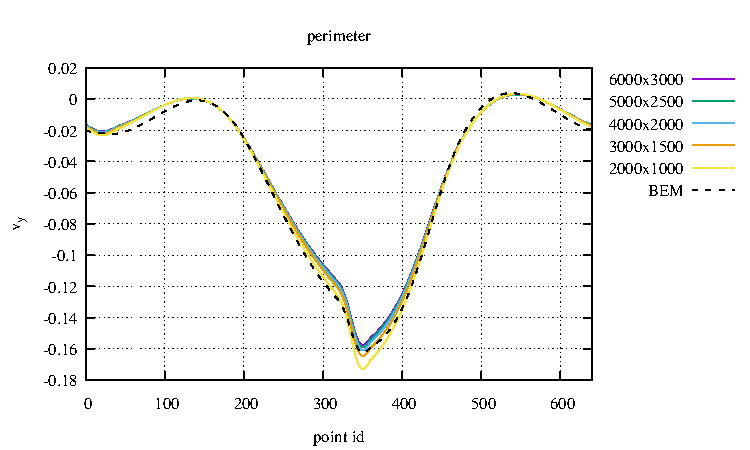
\includegraphics[width=5.7cm]{python_codes/fieldstone_55/gamma100/vy_perimeter}\\
{\captionfont Viscosity contrast $\gamma=100$. From left to right: $u$, zero slab velocity-normalised $u$ 
and $v$ as measured on the spine (top row) and on the perimeter (bottom row). Velocities are normalised by $V_{ref}$}
\end{center}


\begin{center}
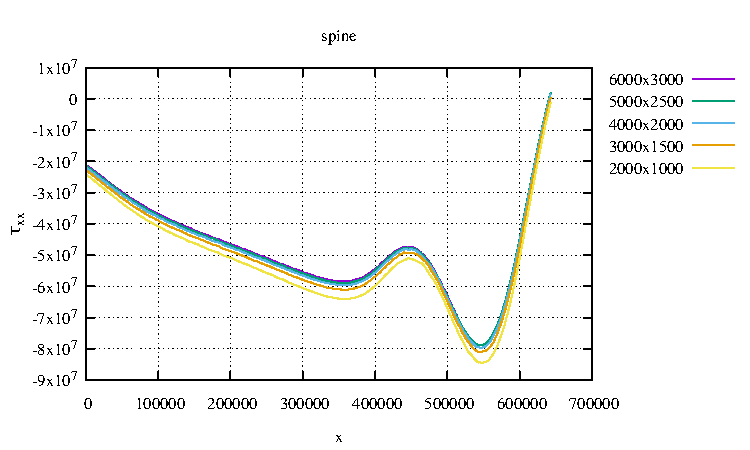
\includegraphics[width=5.7cm]{python_codes/fieldstone_55/gamma100/tau_xx_spine}
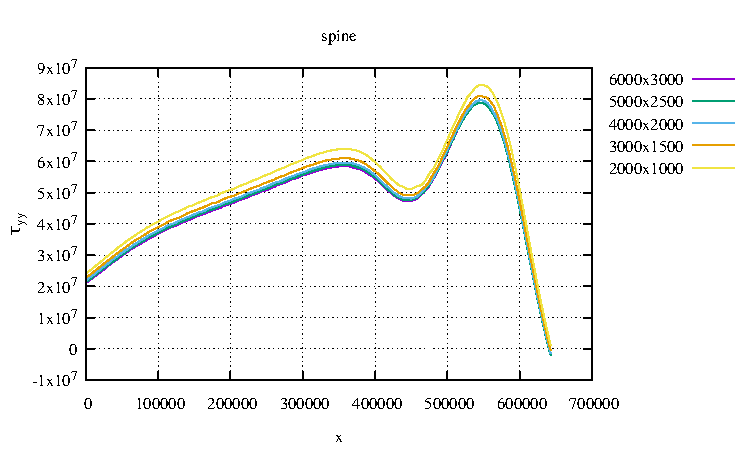
\includegraphics[width=5.7cm]{python_codes/fieldstone_55/gamma100/tau_yy_spine}
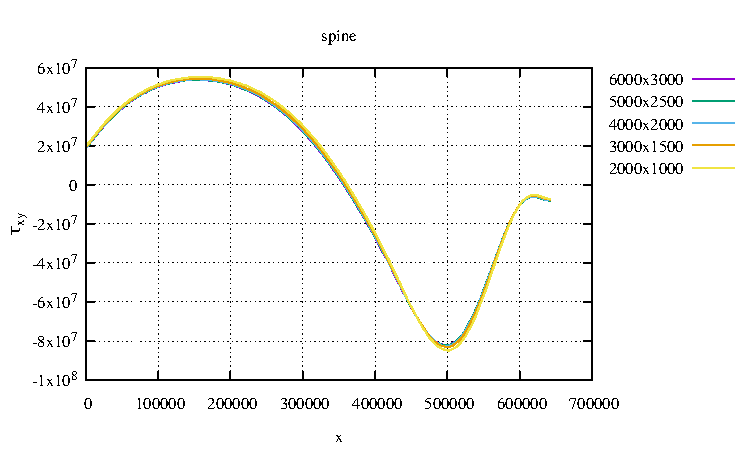
\includegraphics[width=5.7cm]{python_codes/fieldstone_55/gamma100/tau_xy_spine}\\
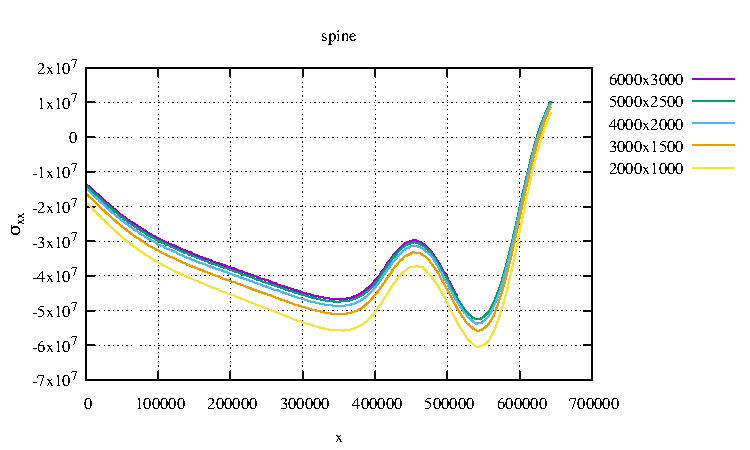
\includegraphics[width=5.7cm]{python_codes/fieldstone_55/gamma100/sigma_xx_spine}
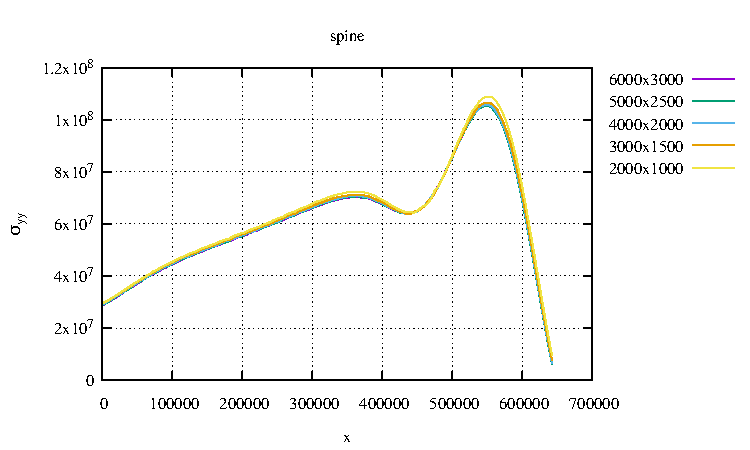
\includegraphics[width=5.7cm]{python_codes/fieldstone_55/gamma100/sigma_yy_spine}
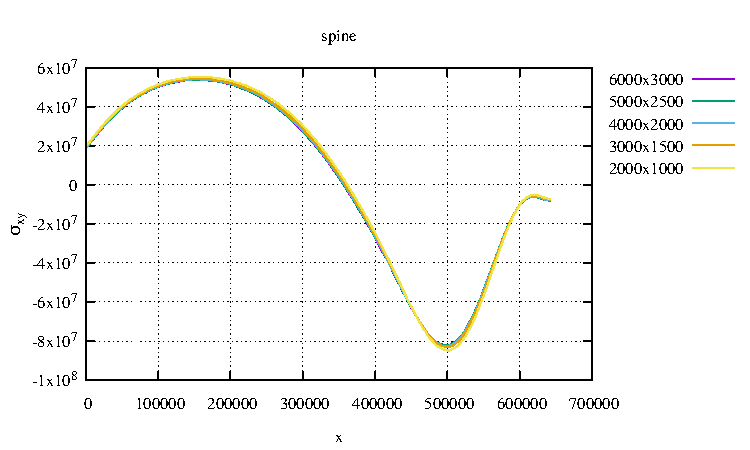
\includegraphics[width=5.7cm]{python_codes/fieldstone_55/gamma100/sigma_xy_spine}\\
{\captionfont Deviatoric and full stress components on the spine of the slab.}
\end{center}

We see that results seem to converge to a domain size-independent profile, for both $u$ and $v$
fields as measured on the spine and on the perimeter of the slab. 

I have also quickly explored the influence of the mesh resolution for a given domain size 
and it appears that the resolution used for these calculations is sufficient to capture 
a resolution independent velocity field.

The question remains as to why BEM results still differ substantially from my high resolution
large domain results.

Neil wrote: ``From the point of view of thin-sheet theory, the dominant stress component
should be $\sigma_{ss}$, where $s$ is the coordinate parallel to the spine. $\sigma_{ss}$
should vary linearly across the plate is deformation is dominated by bending,
and should be constant across the plate if it is dominated by stretching. In the 
flat part of the plate, $sigma_{ss} = \sigma_{xx}$. So your image of $\tau_{xx}$, with
a linear dependence across the flat part, corresponds to bending
deformation. The bending here is so strong because the 
lubrication layer is thick: that allows the slab to bend down the whole interior
of the plate while not undergoing strong bending itself. If possible, it would
probably be a good idea to decrease the lubrication layer thickness from
$0.5 h$ to $0.3 h$ or (better yet) $0.2 h$. ''









\newpage
%----------------------------------------------------------------------
\subsection*{Time evolution with ASPECT}
Finally, we have run this experiment over time with ASPECT (unfortunately viscosities were 100 times 
too small so that the times should be multiplied by 100):
\begin{center}
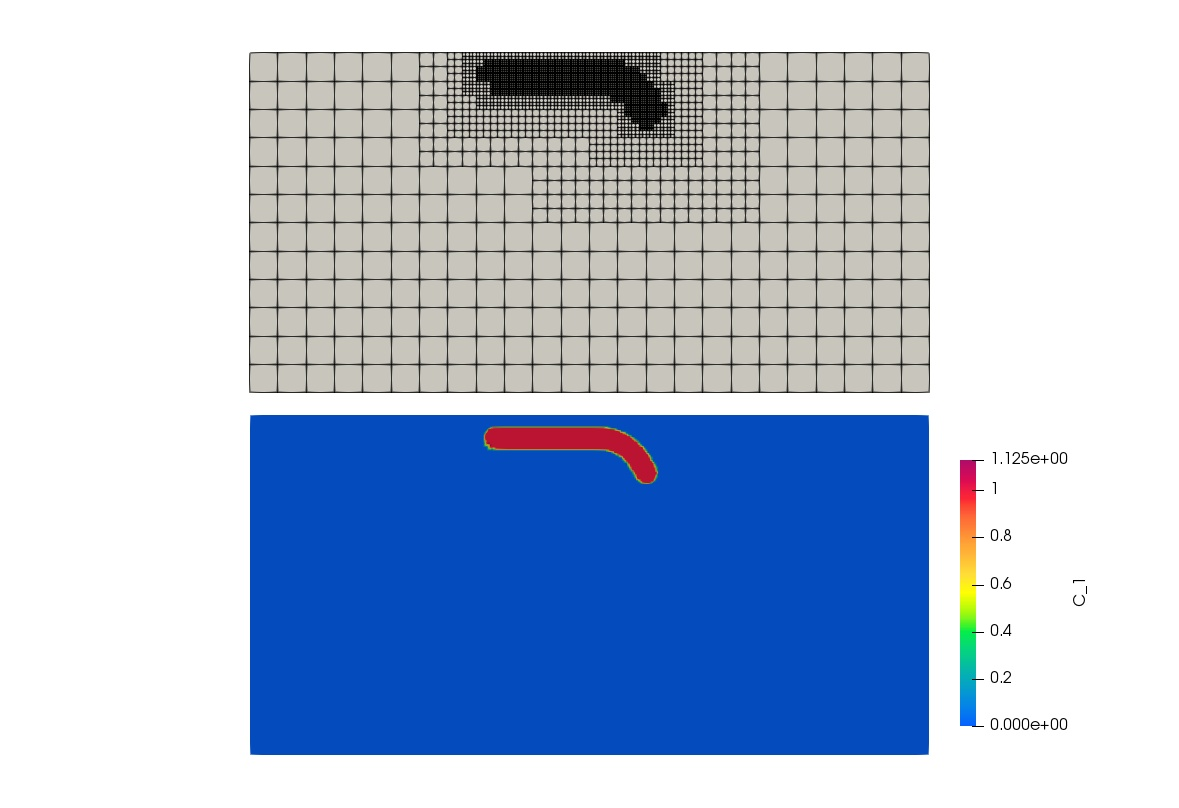
\includegraphics[width=5.26cm]{python_codes/fieldstone_55/images/aspect/grid_comp0000}
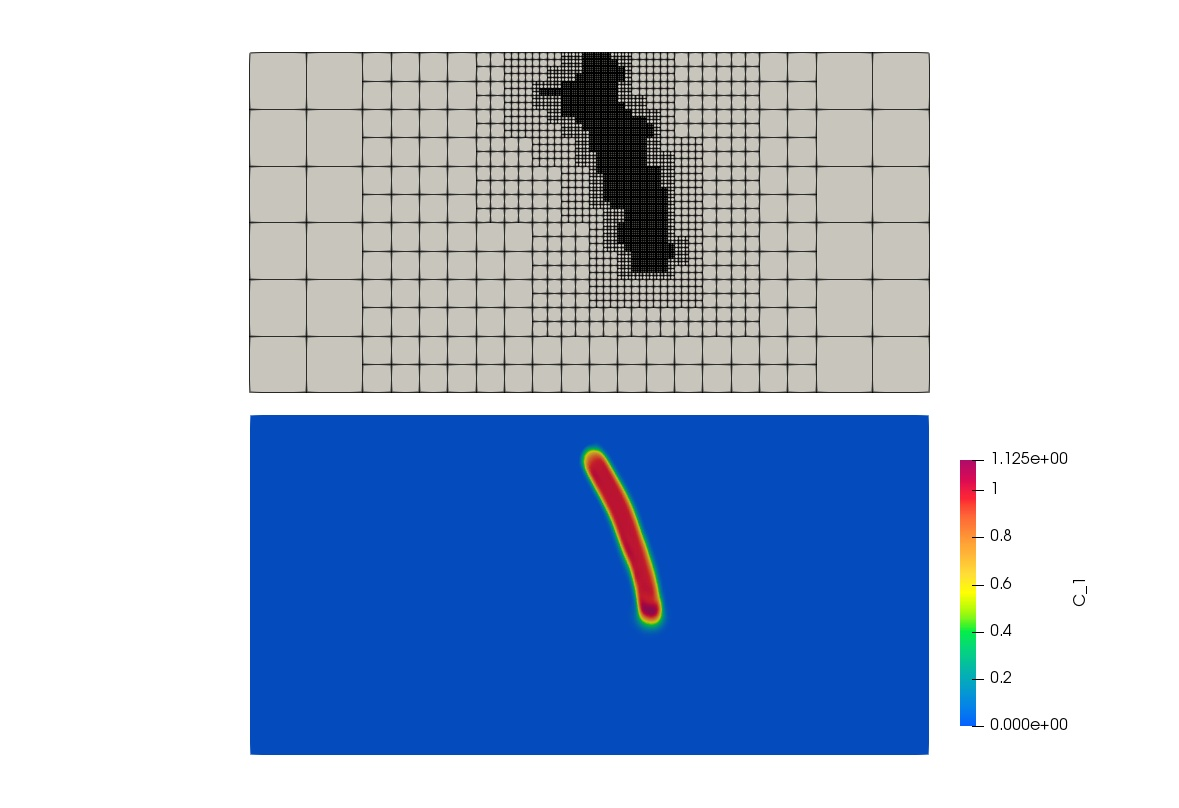
\includegraphics[width=5.26cm]{python_codes/fieldstone_55/images/aspect/grid_comp0090}
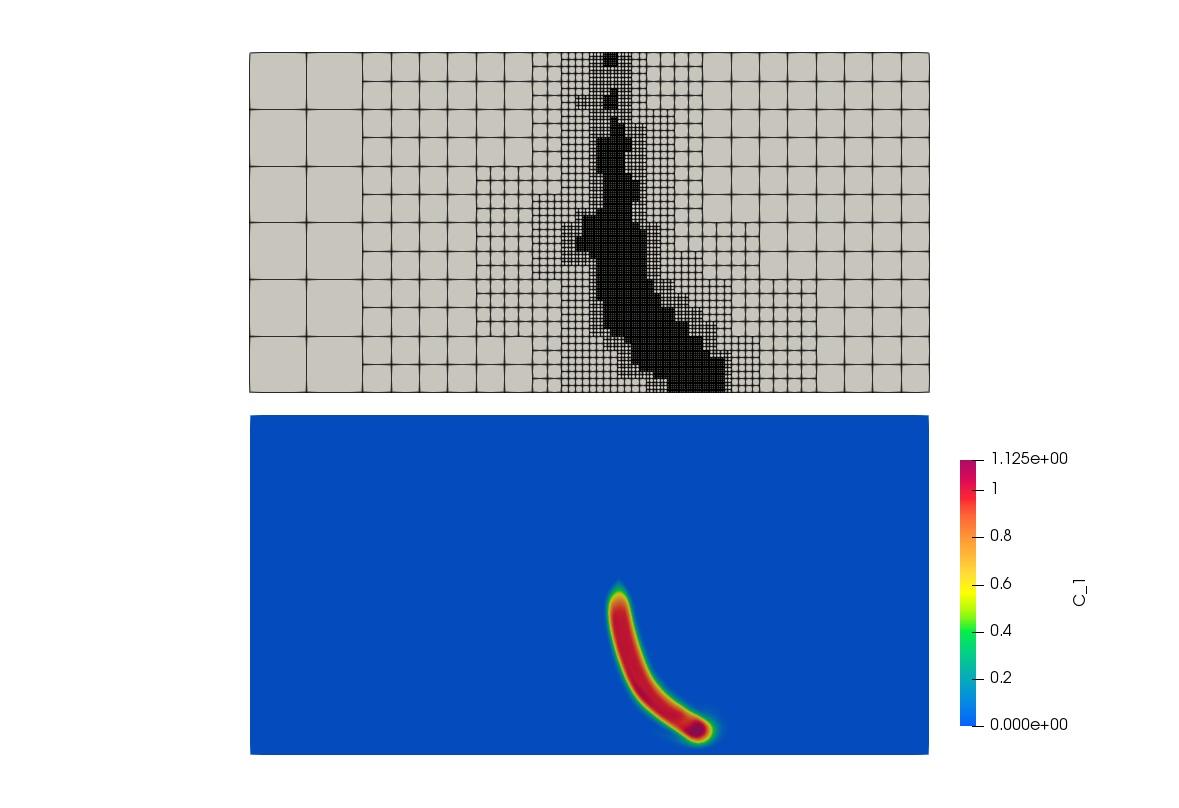
\includegraphics[width=5.26cm]{python_codes/fieldstone_55/images/aspect/grid_comp0180}\\
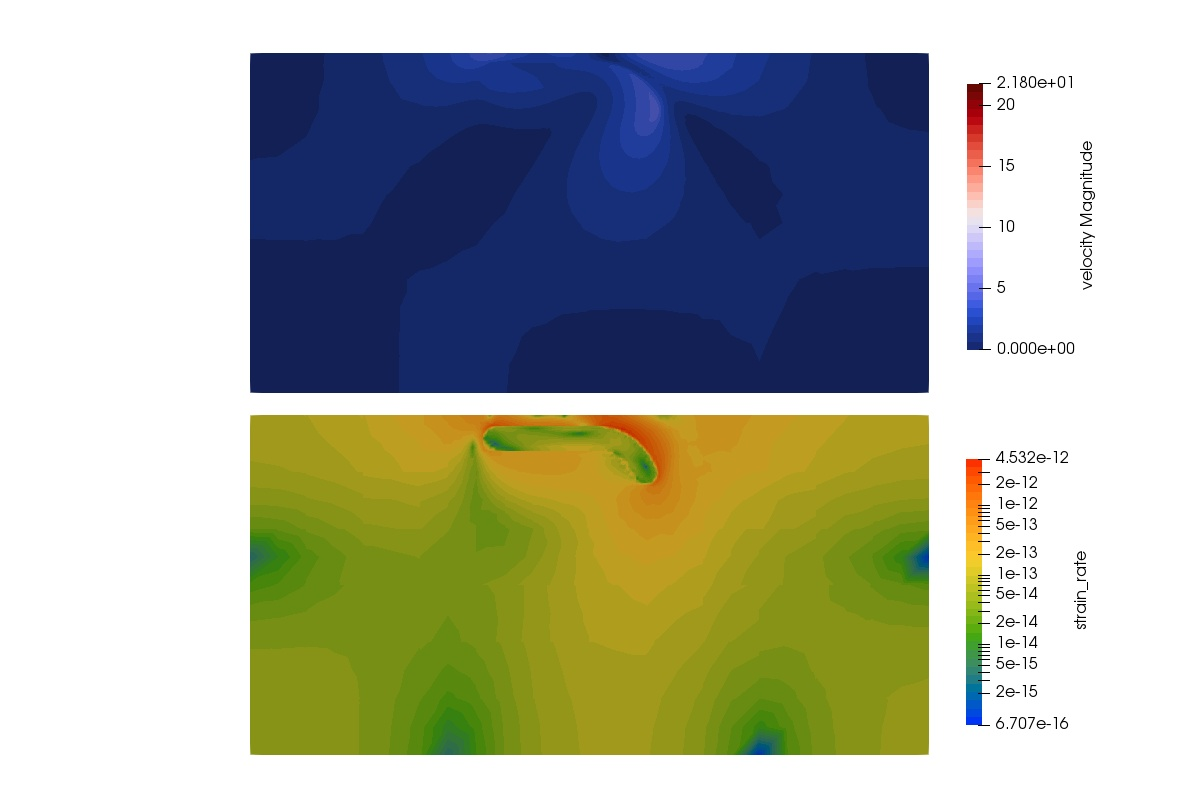
\includegraphics[width=5.26cm]{python_codes/fieldstone_55/images/aspect/vel_sr0000}
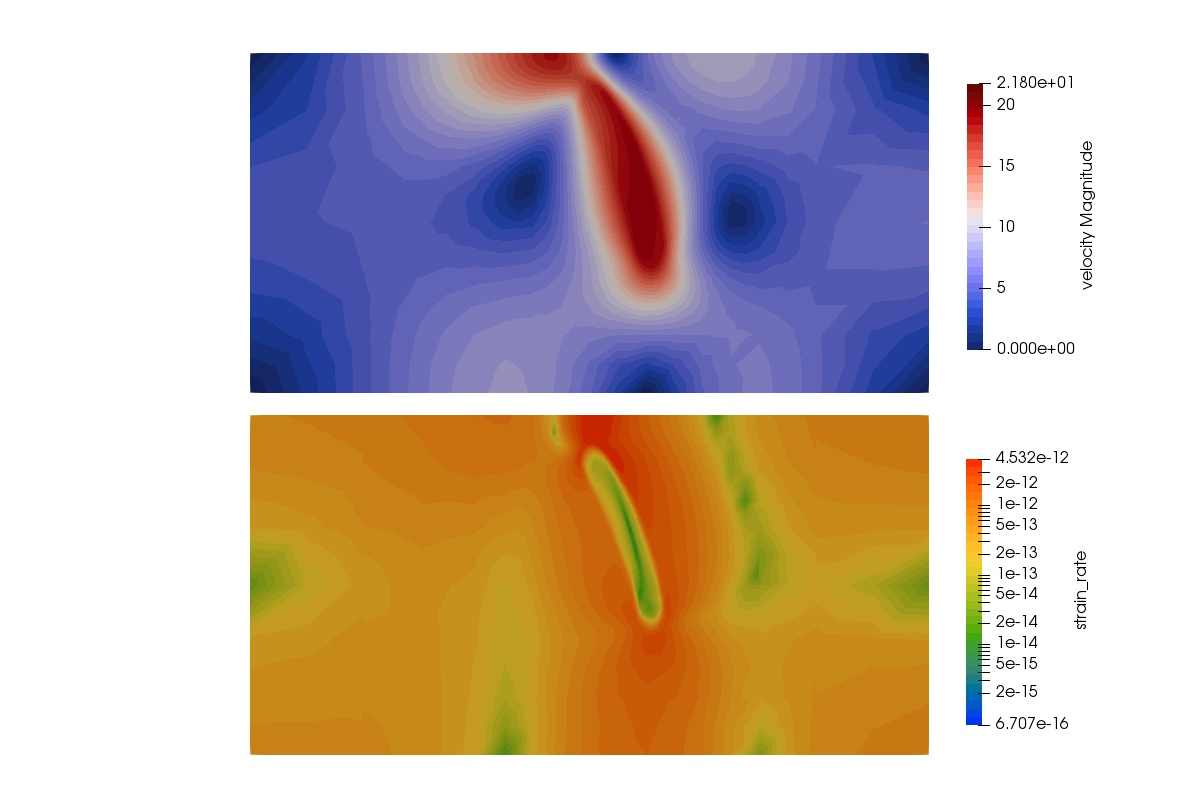
\includegraphics[width=5.26cm]{python_codes/fieldstone_55/images/aspect/vel_sr0090}
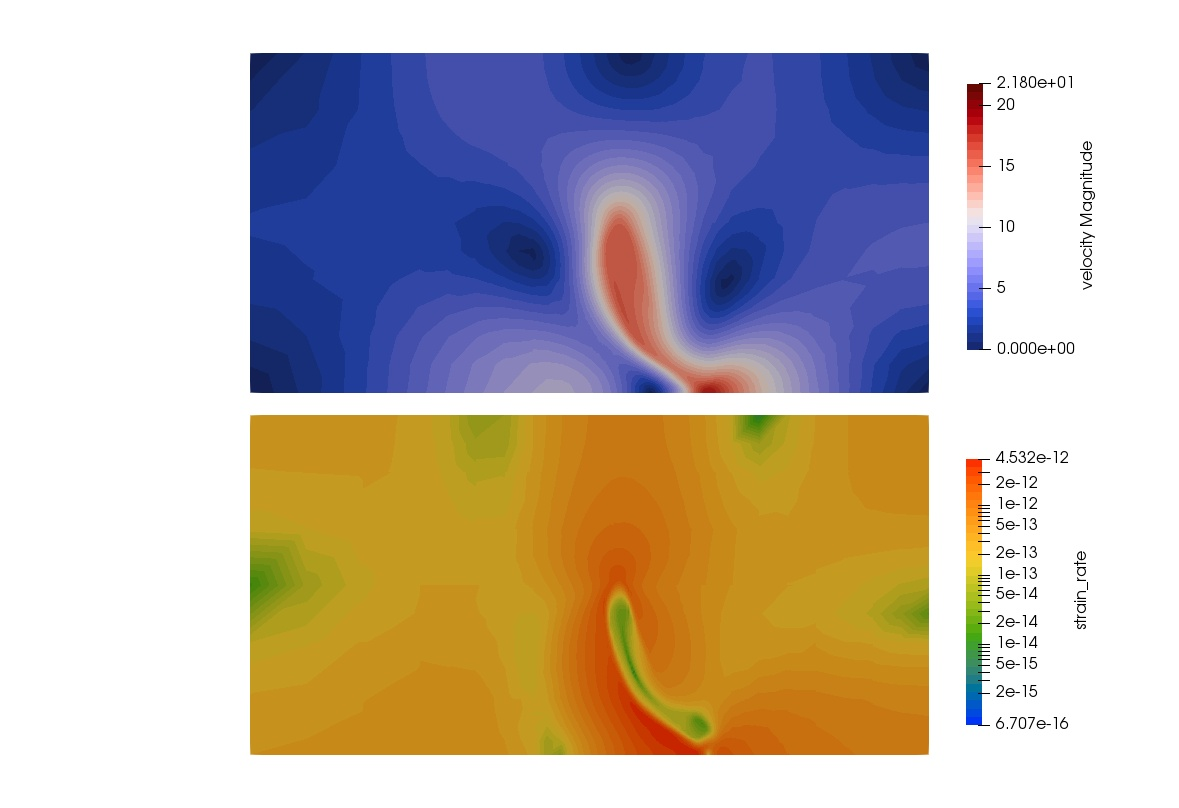
\includegraphics[width=5.26cm]{python_codes/fieldstone_55/images/aspect/vel_sr0180}\\
{\captionfont Left: t=0, middle t=64kyr, right: t=100kyr.}
\end{center}


\begin{center}
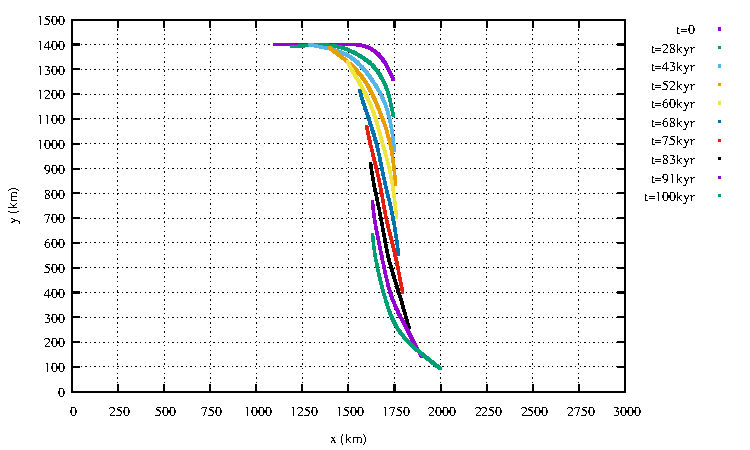
\includegraphics[width=11cm]{python_codes/fieldstone_55/images/mid_evolution}\\
{\captionfont Time evolution of the midline of the slab.}
\end{center}


\begin{center}
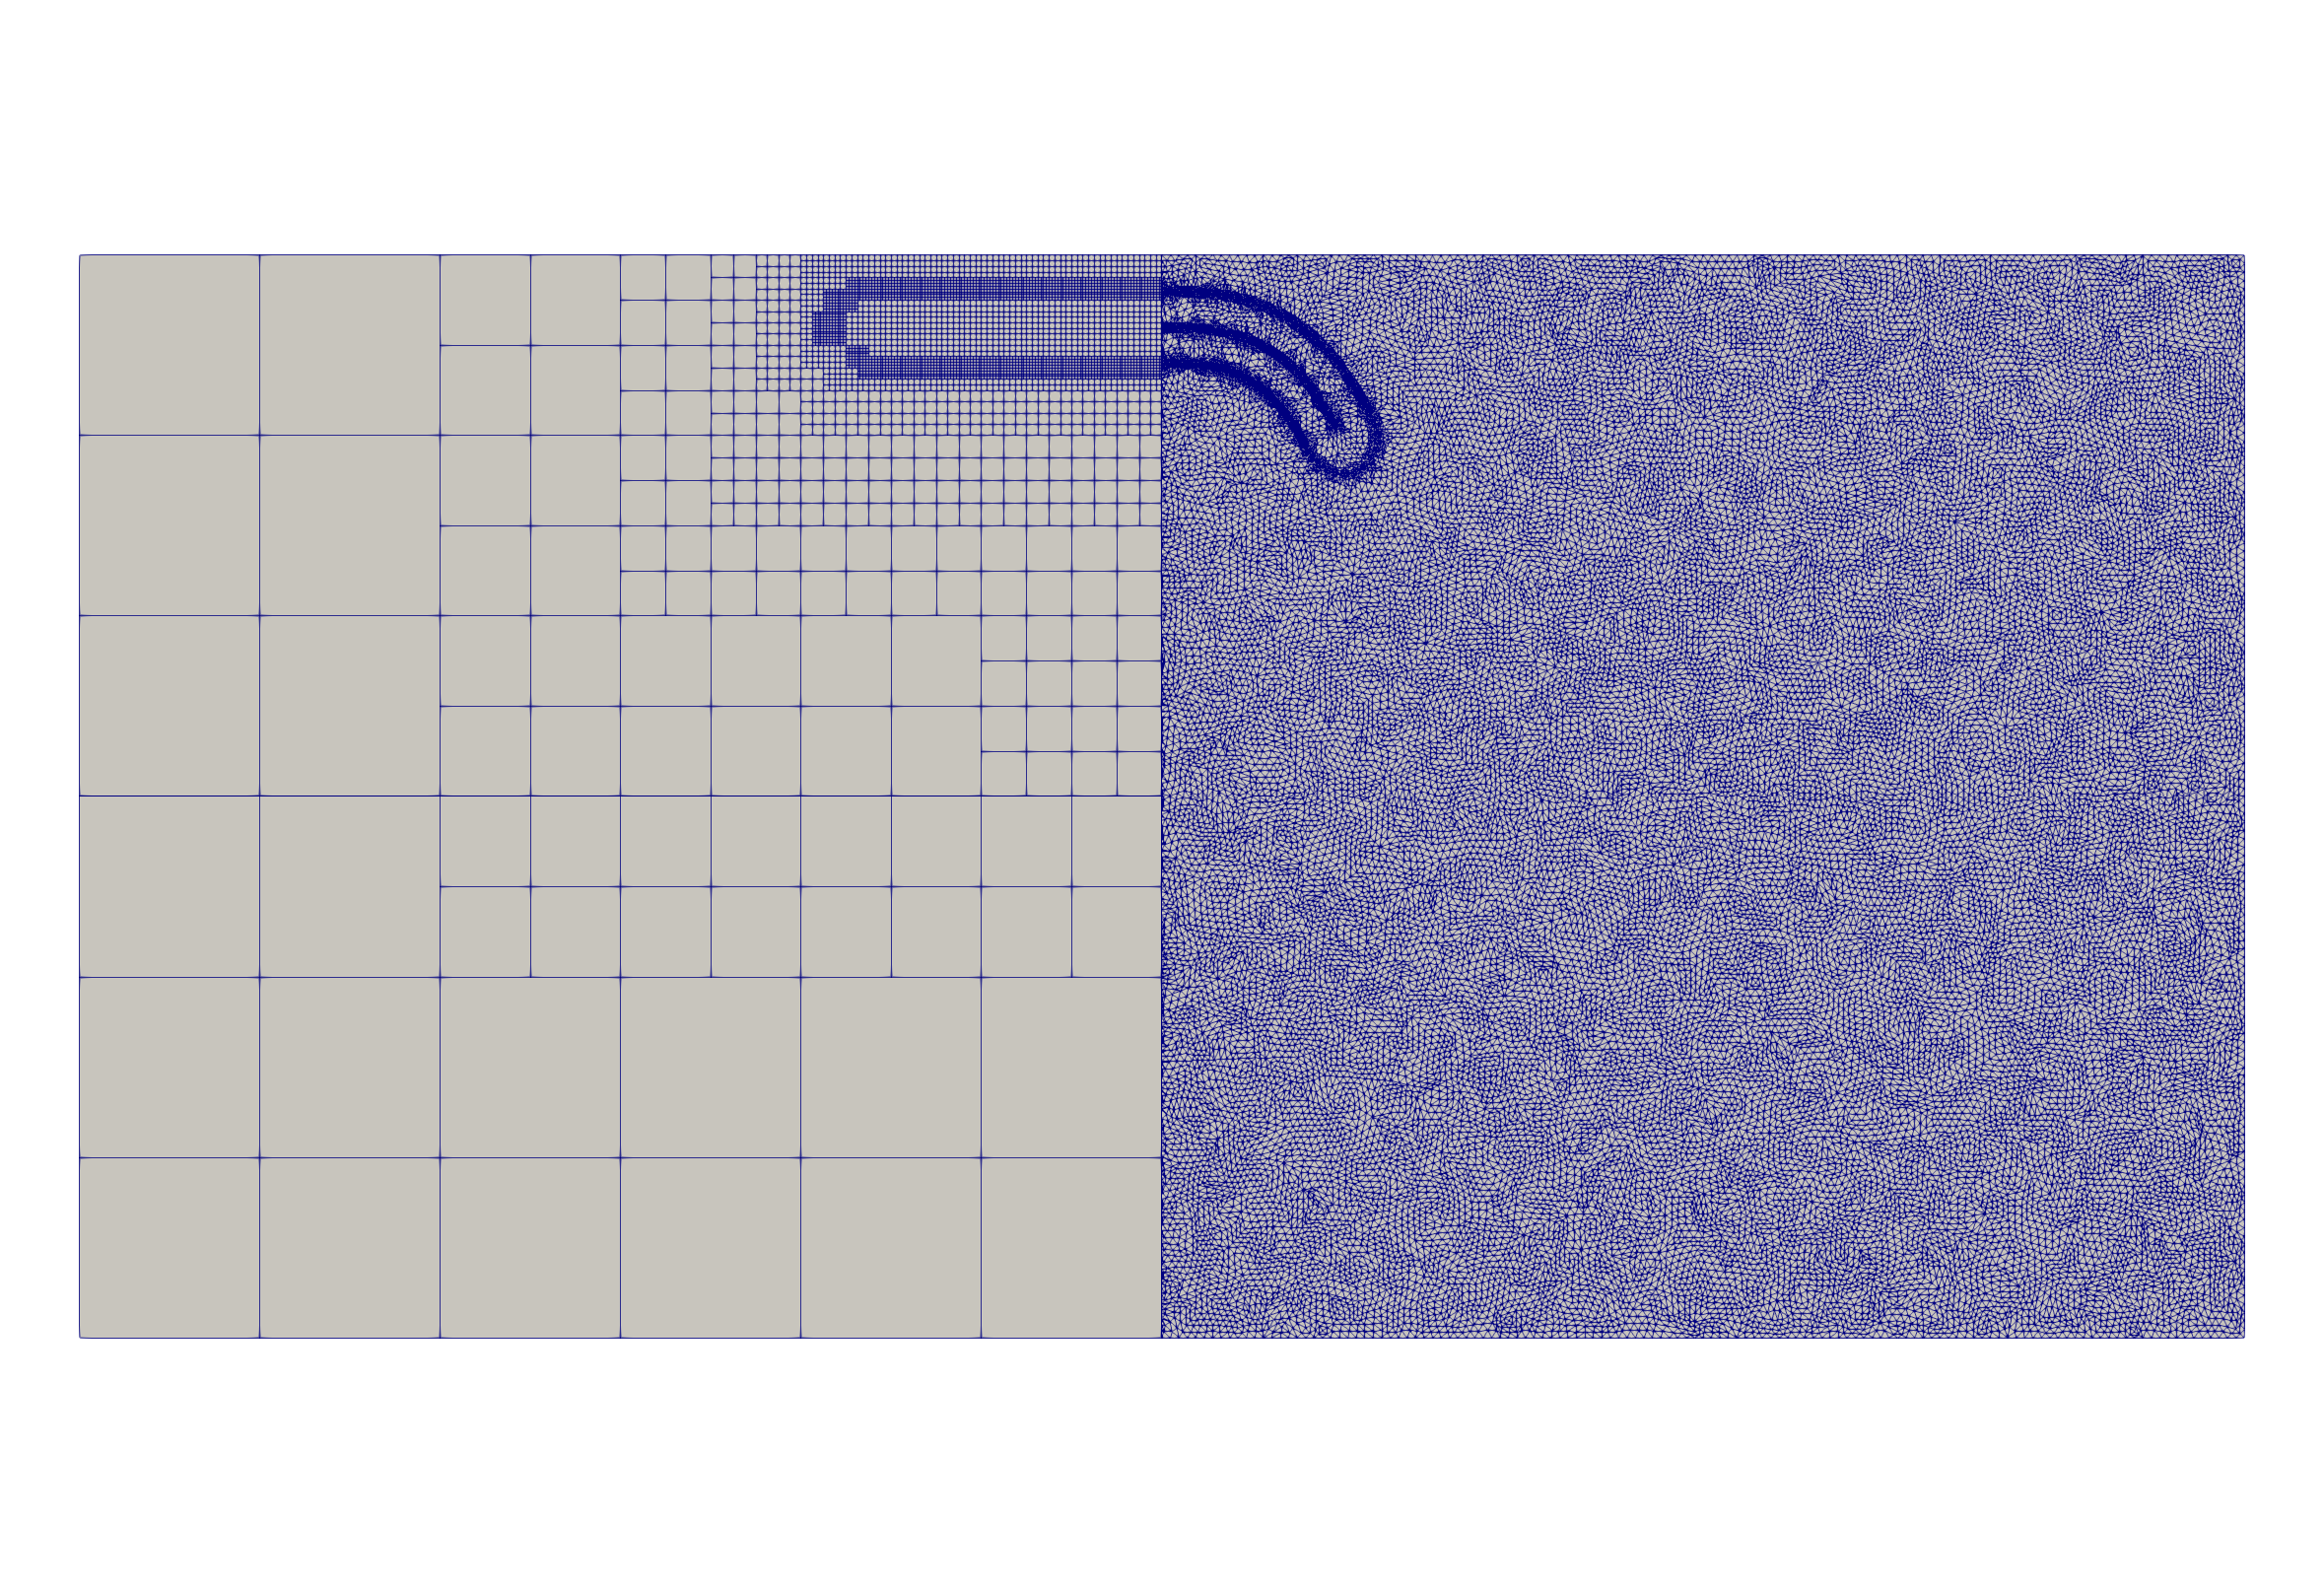
\includegraphics[width=14cm]{python_codes/fieldstone_55/images/meshes}
\end{center}

%area = 2*0.537071*h**2 + (7*h)*h , 80728764230.49994 with h=100km

\vspace{3cm}

%\begin{center}
%\includegraphics[width=7cm]{python_codes/fieldstone_55/images/spine_Us}
%\includegraphics[width=7cm]{python_codes/fieldstone_55/images/spine_Ws}\\
%{\scriptsize Parallel and perpendicular velocity to midsurface. $s$ is measured from 
%left to right on the midsurface and excludes the rounded edges of the slab.}
%\end{center}





Literature: \cite{fogm14}
